%%%%%%%%%%%%%%%%%%%%%%%%%%%%%%%%%%%%%%%%%%%%%%%%%%%%%%%%%%%%%
%% SAVE ME %%%%%%%%%%%%%%%%%%%%%%%%%%%%%%%%%%%%%%%%%%%%%%%%%%%%%%%%%%%%%
\documentclass[]{article}
\setlength{\oddsidemargin}{1pt}
\setlength{\evensidemargin}{1pt}
\usepackage{amssymb,mathtools,tikz}
\usepackage {stmaryrd}
\usepackage[ligature, inference]{semantic}
\textwidth=16cm
\marginparwidth = 5pt
\oddsidemargin = 1pt

\newcommand{\setB}{{\mathord{\mathbb B}}}
 
\newcommand {\wps}[0]{wp}
\newcommand {\wlps}[0]{wlp}
 \newcommand {\etc}[0]{etc.}
\newcommand {\eg}[0]{e.g.}
\newcommand {\ie}[0]{i.e.}
\newcommand {\trr}[0]{Tr^{c}}
\newcommand {\vab}[0]{vA_B}

\newcommand {\AbsLH}[2]{\, _{#1}{Abs}_{#2}}

\newcommand {\parp} [1]{ \hspace*{-0.5ex}||_{#1} \hspace*{-0.5ex}}
\newcommand {\parpp} [1]{ ||_{#1} }
\newsavebox{\mytbx}  
\newsavebox{\myttbx}  
\newsavebox{\mybx}  
\newsavebox{\mybxx}  
\newsavebox{\mybxxx}  
\newcommand {\mythin}[4]
    {
\savebox{\mybx}{#1}  
\settowidth{\dslen}{\usebox{\mybx}}     
 \addtolength{\dslen}{#4}
\begin{floatingfigure}[r]{\dslen}
\hspace*{#4}\hspace*{-1ex}\usebox{\mybx}
 \caption{#2}   
  \label{#3}
\end{floatingfigure} 
    }
%\newsavebox{\mybx}  
\newcommand {\myfloat}[3]
    {
\savebox{\mybx}{#1}  
\settowidth{\dslen}{\usebox{\mybx}}     
\begin{floatingfigure}[r]{\dslen}
\noindent
\usebox{\mybx} \vspace{-3ex}
  \caption{\ #2}   
  \label{#3}
\end{floatingfigure} 
    }
\newcommand {\oldfloat}[3]
    {
\savebox{\mybx}{#1}  
\settowidth{\dslen}{\usebox{\mybx}}     
\begin{floatingfigure}[r]{\dslen}
\noindent
\usebox{\mybx}
  \caption{\ #2}   
  \label{#3 }
\end{floatingfigure} 
    }
\newcommand {\myfloatwo}[2]
    {
\savebox{\mybx}{#1}  
\settowidth{\dslen}{\usebox{\mybx}}     
\begin{floatingfigure}[r]{\dslen}
\noindent
\usebox{\mybx}
  \label{#2}
\end{floatingfigure} 
    }

\newcommand {\myfig}[3]
    {
\savebox{\mybx}{#1} 
    \settowidth{\dslen}{\usebox{\mybx}}
   \begin{figure}[!htb]
   \begin{center}
     \begin {minipage}{\dslen}{#1}\end{minipage}
     \caption{\ #2}
\label{#3}
   \end{center}
   \end{figure}
     }
\newcommand {\myfigtwo}[4]
    {
\savebox{\mybx}{#1} 
    \settowidth{\dslen}{\usebox{\mybx}}
   \begin{figure}[!htb]
   \begin{center}
     %\fbox{
    \begin {minipage}{\dslen}{#1}\end{minipage}
    %}
 \savebox{\mybx}{#4} 
    \settowidth{\dslen}{\usebox{\mybx}}
       %\fbox{
     \begin {minipage}{\dslen}{#4}\end{minipage}
      %}
   \caption{\ #2} 
\label{#3}
   \end{center}
   \end{figure}
    }
\newcommand {\myfigf}[4]
    {
\savebox{\mybx}{#1} 
    \settowidth{\dslen}{\usebox{\mybx}}
   \begin{figure}[!htb]
   \begin{center}
     \begin {minipage}{\dslen}{#1}

    \footnotesize{#4}\end{minipage}
      \caption{\ #2}
\label{#3}
   \end{center}

   \end{figure}
    }
    
\newcommand {\myfigb}[3]
    {
\savebox{\mybx}{#1}  
\settowidth{\dslen}{\usebox{\mybx}}     
\noindent
\begin{figure}[b]
\noindent
\begin{center}
\makebox[\dslen][c] {
\usebox{\mybx}}  \caption{#2}   
  \label{#3}
\end{center}
\end{figure} 
    }

\newcommand {\Arop} [4] 
{\ensuremath{{#1}{{\stackrel{#2}{\Longrightarrow}}_{#4}}{#3} }}

%%%%%%%%%%%%
% Z sequence-filter
\newcommand{\zfilter} [2] { {#1} \upharpoonright{#2}}

%\usepackage {ifthen}
%\usepackage [dvips] {graphics}
\newlength{\dslen}
\newlength{\dslena}
\newlength{\dslenb}
\newcommand {\overo} [1] {\widehat{#1}}


\newsavebox{\mytab}
\newcommand {\mybox} [1]
    {
\settowidth{\dslena}{#1}
  \raisebox{\dslena}{#1}
   }
\newcommand {\parsyn} [1] {\stackrel{\parallel}{\scriptstyle #1}}
%\newcommand {\parsyn} [1] {\parallel_{\vspace{1ex}\hspace{-1ex}\scriptstyle #1}}
\newcommand {\refadt} [0] {Ref_{s}}
\newcommand {\zscol} [0] {\comp}
\newcommand {\scol} [0] {;\hspace{-0.4em}}
\newcommand {\sscol} [0] {;\hspace{-0.2em}}
\newcommand {\sfa} [0] {\sf{a}}
\newcommand {\sfb} [0] {\sf{b}}
\newcommand {\sfc} [0] {\sf{c}}
\newcommand {\citepa} [0] {\cite{Ros97,Mil89,BaW90,Hen88b}}
\newcommand {\hplu} [0] {\ensuremath{\widehat{+}}}
\newcommand {\hpar} [0] {\ensuremath{\widehat{\parallel_{S}}}}
\newcommand {\htau} [0] {\ensuremath{\widehat{\tau}}}
\newcommand {\hdelta} [0] {\ensuremath{\widehat{\delta}}}
\newcommand {\hseq} [0] {\ensuremath{\widehat{\hspace*{0.5ex}; }}}
\newcommand {\hcon} [0] {\ensuremath{\widehat{[\_]}}}

\newcommand {\notangle} [0] {\ensuremath{\hspace*{0.1em}\angle \hspace*{-0.8em}\diagdown}}

\newcommand {\leftproj} [1] {\stackrel{\scriptstyle \gets }{#1}}
\newcommand {\rightproj} [1] {\stackrel{\scriptstyle \to }{#1}}
\newcommand {\pretotal} [1] {\stackrel{\scriptstyle \heartsuit}{#1}}
\newcommand {\lifttotal} [1] {\stackrel{\scriptstyle \bullet}{#1}}
\newcommand {\lsemantics} [0] {\lbrack\mkern-3mu\lbrack}
\newcommand {\rsemantics}     [0] {\rbrack\mkern-3mu\rbrack}

\newcommand {\plcsp}[1] {\ensuremath{{\parallel \atop{\scriptscriptstyle #1}}}}

\newcommand {\parcsp}     [1] {\ensuremath{
 \settowidth{\dslen}{/{#1}}
{\hspace{-\dslen} {\hspace{\dslen}{\sf VM}\parallel{\sf Rob}/{#1} \atop{\scriptscriptstyle #1}}}}}
\newcommand {\partwocsp}     [2] {\ensuremath{
 \settowidth{\dslen}{{#2}}
{\hspace{-\dslen} {\hspace{\dslen}(\_\parallel\_)/{#2} \atop{\scriptscriptstyle #1}}} }}


\newcommand {\absto}[1] {\ensuremath{\stackrel{#1}{\Longrightarrow}} }
%\newcommand {\mylgc} [3] {\ensuremath{
%\settowidth{\dslen}{\mbox {${#1}$}}
%\settowidth{\dslena}{\mbox {${#2}$}}
%\ifthenelse{\dslen < \dslena}{\setlength{\dslena}{\dslen}}{}
%\parbox[t]{\dslen}{\underline{#1} {#2}}
%\settodepth{\dslena}{\mbox ${#3}$}
%\raisebox{\dslena}{${#3}$} }}

\newcommand {\mylogic} [3] {
\xymatrix@R=0pt@C=0pt@M=0pt{&{#1} \\
\ar@{-}[rr] &&\hspace{1.0ex}{#3}\hspace{1.0ex}\\
 &{#2}}}

%\newcommand {\mylgcy} [3] {
%\settowidth{\dslen}{\mbox{#1}}
%\settowidth{\dslena}{\mbox{#2}}
%\ifthenelse{\dslen < \dslena}
%{\parbox[t]{\dslena}{\underline{\makebox[\dslena]{#1}} {#2}}}
%{\parbox[t]{\dslen}{\underline{#1} \makebox[\dslen]{#2}}}
%%\settodepth{\dslena}{\mbox {#3}}
%\raisebox{-1.0ex}{#3} }

%\newcommand {\mylgcyy} [5] {
%\settowidth{\dslen}{\mbox{#1}}
%\settowidth{\dslena}{\mbox{#2}}
%\settowidth{\dslenb}{\mbox{#4}}
%\ifthenelse{\dslen < \dslena}
%{\setlength{\dslen}{\dslena}}
%{}
%\ifthenelse{\dslen < \dslenb}
%{\setlength{\dslen}{\dslenb}}
%{}
%{\begin{minipage}[b]{\dslen}
%\parbox[t]{\dslen}{\underline{\makebox[\dslen]{#1}}
%\underline{\makebox[\dslen]{#2}}
%\raisebox{-1.0ex}{#3}} \\ \mbox{} \end{minipage}
%\\ \parbox[t]{\dslen}{#4}\raisebox{-1.0ex}{#5}}}

\newcommand {\ct} [1] {\stackrel{\scriptstyle \circ \hspace*{-0.2ex} \to  }{T_{#1}}}

%%%\newcommand {\arocel}[3] {\ensuremath{
%%%{#1}\buildrel {#2} \over {\circ \hspace*{-1.0ex} - \hspace*{-1.1ex} - \hspace*{-1.1ex} \to }{#3} }}

%%%\def\rightcircfill{$\mathsurround=0pt \circ \mkern-2.4mu
%%%\\cleaders\hbox{$\mkern-2mu \mathord- \mkern-2mu$}\hfill
%%%\\mkern-6mu \mathord\to $}

%%%\\newcommand {\arocel}[3] {\ensuremath{
%%%\\settowidth{\dslen}{\hbox {${#2}$\hspace{1ex}}}
%%%\{#1}\buildrel {#2} \over {\hbox to \dslen{\rightcircfill}}{#3} }}



\def\rightharpfill{$\mathsurround=0pt - \mkern-6mu
\cleaders\hbox{$\mkern-2mu \mathord- \mkern-2mu$}\hfill
\mkern-6mu \mathord\rightharpoondown$}

\def\Rightmapfill{$\mathsurround=0pt \models \mkern-6mu
\cleaders\hbox{$\mkern-2mu \mathord= \mkern-2mu$}\hfill
\mkern-6mu \mathord\Rightarrow$}

\def\Rightarrowfill{$\mathsurround=0pt \mathord= \mkern-6mu
\cleaders\hbox{$\mkern-2mu \mathord= \mkern-2mu$}\hfill
\mkern-6mu \mathord\Rightarrow$}

\newcommand {\AroL}[4] {\ensuremath{
\settowidth{\dslen}{\hbox {$\langle{#2},{#4}\rangle$}}
{#1}\buildrel \langle{#2},{#4}\rangle \over {\hbox to \dslen{\Rightarrowfill}}{#3} }}

\newcommand {\arotwop} [6]
{\ensuremath{{#1}{\stackrel{#2}{\longrightarrow_{#6}}}{#3}{\stackrel{#4}{\longrightarrow_{#6}}}{#5} }}



\newcommand {\aro} [3]
{\ensuremath{{#1}{\stackrel{#2}{\longrightarrow}}{#3} }}

\newcommand {\arotwo} [5]
{\ensuremath{{#1}{\stackrel{#2}{\longrightarrow}}{#3}{\stackrel{#4}{\longrightarrow}}{#5} }}

\newcommand {\aroeltwo}[5] {\ensuremath{
\settowidth{\dslen}{\hbox {${#2}$}}
\settowidth{\dslena}{\hbox {${#4}$}}
{{#1}\buildrel {#2\hspace{-0.5ex}} \over {\hbox to \dslen{\rightarrowfill}}{\hspace{-0.5ex}#3}\buildrel {#4\hspace{-0.5ex}} \over {\hbox to \dslena{\rightarrowfill}}{\hspace{-0.5ex}#5} }}}

\newcommand {\Bmath}[0]{\ensuremath{\mathbb B}}
\newcommand {\Emath}[0]{\ensuremath{\mathbb E}}
\newcommand {\Pmath}[0]{\ensuremath{\mathbb P}}


\newcommand {\Aro} [3]
{\ensuremath{{#1}{\stackrel{#2}{\Longrightarrow}}{#3} }}

\newcommand {\aroleft} [3]
{\ensuremath{{#1}{\stackrel{#2}{\longleftarrow}}{#3} }}
\newcommand {\arew} [1] {\ensuremath{\stackrel{#1}{\leadsto}}}
\newcommand {\defeq}  {\ensuremath{ \hspace*{0.5em}
\stackrel{\mathrm{def}}{=} \hspace*{0.5em}} }

\newtheorem {mypdef}      {Definition}
\newtheorem {myplemma}     {Lemma} 
\newtheorem {myptheorem}  {Theorem}
\newtheorem {mypass}      {Assumption}
%\newtheorem {myprwa}      {Real World Assumption}
\newtheorem {mypprop}      {Property}
%\newtheorem {myptheorem} [mypdef] {Theorem}

\newcommand {\sref} [1] {Section~\ref{sec:#1}}
\newcommand {\aref} [1] {Assumption~\ref{ass:#1}}
\newcommand {\dref} [1] {Definition~\ref{def:#1}}
\newcommand {\pref} [1] {Property~\ref{pro:#1}}
\newcommand {\lref} [1] {Lemma~\ref{lem:#1}}
\newcommand {\tref} [1] {Theorem~\ref{thm:#1}}
\newcommand {\fref} [1] {Fig.~\ref{fig:#1}}
%\newcommand {\rwaref} [1] {Real World Assumption~\ref{rwa:#1}}

\newcommand {\myproof} {\noindent {\bf Proof\hspace{1em} }}
\newcommand {\mylend} {\noindent \ensuremath{\hfill\bullet}}
\newcommand {\mydend} {\noindent \ensuremath{\hfill{\bullet}}}
\newcounter{lno}
\newcounter{listno}
\newcommand {\pcm}
{\ensuremath{\vert\hspace{-0.3ex}\vert\hspace{-0.3ex}\vert} }
\newcommand {\myprog} [1]
    {\begin{verbatim} \include {#1} \end{verbatim} }
\newcommand {\aroelp}[4] {\ensuremath{
\settowidth{\dslen}{\hbox {${#2}\hspace{0.5em}$}}
{#1}\buildrel {#2} \over {\hbox to \dslen{\rightarrowfill}}_{#4}{#3} }}

\newcommand {\harp}[3] {\ensuremath{
\settowidth{\dslen}{\hbox {${#2}\hspace{0.5em}$}}
{#1}\buildrel {#2} \over {\hbox to \dslen{\rightharpfill}}{#3} }}


\newcommand {\saroelp}[4] {\ensuremath{\scriptstyle{
\settowidth{\dslen}{\hbox {${#2}$\hspace{-0.5em}}}
{#1}\buildrel {#2} \over {\hbox to \dslen{\rightarrowfill}}_{#4}{#3} }}}
\newcommand {\aroelps}[4] {\ensuremath{
\settowidth{\dslen}{\hbox {${#2}\hspace{-2.0em}$}}
{#1}\buildrel {#2} \over {\hbox to \dslen{\rightarrowfill}}_{#4}{#3} }}

\newcommand {\Aroel}[3] {\ensuremath{
\settowidth{\dslen}{\hbox {${#2}$}}
{#1}\buildrel {#2} \over {\hbox to \dslen{\Rightarrowfill}}{#3} }}

\newcommand {\aroel}[3] {\ensuremath{
\settowidth{\dslen}{\hbox {${#2}$}}
{#1}\buildrel {#2\hspace{-0.5ex}} \over {\hbox to \dslen{\rightarrowfill}}{\hspace{-0.5ex}#3} }}


\newcommand {\arop}
[4]{\ensuremath{{#1}{\stackrel{#2}{\longrightarrow}_{#4}}{#3} }}

\newcommand {\notaro}
[3]{\ensuremath{{#1}{\stackrel{#2}{\,\,\not\!\!\longrightarrow}}{#3} }}
\newcommand {\notarop}
[4]{\ensuremath{{#1}{\stackrel{#2}{\,\,\not\!\!\longrightarrow}_{#4}}{#3 }
}}
\newcommand {\compress} {\setlength{\itemsep}{0cm}
\setlength{\parsep}{0cm}
\setlength{\topsep}{0cm}}
\newcommand {\myfigfour}[4]
    {
\savebox{\mybx}{#1} 
    \settowidth{\dslen}{\usebox{\mybx}}
   \begin{figure}[!htb]
   \begin{center}
     \begin {minipage}{\dslen}{#1}

    \footnotesize{#4}\end{minipage}
      \caption{#2}\label{#3}
   \end{center}

   \end{figure}
    }






\newcommand {\Arx}[4] {\ensuremath{
{#1}\buildrel \langle{#2},{#4}\rangle \over {\Rightarrowfill{#2}{#4}}}{#3} }

 %%%%%%%%%%%%%%%%%%%%%%%%%%%%%%%%%%%%%%%%%%%%%%%%%
\usepackage[USenglish]{babel} %francais, polish, spanish, ...
%\usepackage[T1]{fontenc}
%\usepackage[ansinew]{inputenc}
%\usepackage{mnsymbol}
\usepackage{hyperref}
%\usepackage{lmodern} %Type1-font for non-english texts and characters
\usepackage{xcolor}


%% Packages for Graphics & Figures %%%%%%%%%%%%%%%%%%%%%%%%%%
\usepackage{graphicx} %%For loading graphic files

%% Math Packages %%%%%%%%%%%%%%%%%%%%%%%%%%%%%%%%%%%%%%%%%%%%
\usepackage{amsmath}
\usepackage{amsthm}
\usepackage{amsfonts}
%\usepackage{b2latex}

%% Line Spacing %%%%%%%%%%%%%%%%%%%%%%%%%%%%%%%%%%%%%%%%%%%%%
%\usepackage{setspace}
%\singlespacing        %% 1-spacing (default)
%\onehalfspacing       %% 1,5-spacing
%\doublespacing        %% 2-spacing



\newcounter{dead1}
\newcounter{dead2}


%%%%%%%%%%%%%%%%%%%%%%%%%%%%%%%%%%%%%%%%%%%%%%%%%%%%%%%%%%%%%
%% DOCUMENT
%%%%%%%%%%%%%%%%%%%%%%%%%%%%%%%%%%%%%%%%%%%%%%%%%%%%%%%%%%%%%
\begin{document}

\pagestyle{empty} %No headings for the first pages.


%% Title Page %%%%%%%%%%%%%%%%%%%%%%%%%%%%%%%%%%%%%%%%%%%%%%%
%% ==> Write your text here or include other files.

%% The simple version:
\title{Transpower Formal verification}
\author{David Streader}

\pagestyle{plain} %Now display headings: headings / fancy / ...

{\LARGE \bf
\begin{center}
Modelling  and model checking interactive programs
\end{center}
}

%$\xRightarrow{\text{helloxxxxxx}}$


Here we are interested in programs that interact with the world around them and need not terminate to be useful. These programs  run concurrently with the world around them. The formal modelling   of such programs has been achieved in a wide variety of styles. Unfortunately each style of modelling take a significant effort to understand in detail and consequently most people become an \emph{expert} in only one way of modelling. Each of the modelling styles  is predicated on a set of assumptions that are commonly unvoiced and hence comparison between styles is far from easy.



To help formalise this we  model programs that can themselves be concurrent. The class of such concurrent programs is very varied  and many distinct styles of analysis appear in the literature.  We find it helpful to decompose these concurrent programs into two broad, overlapping,  classes \emph{State based} and \emph{Event based}.

Here we  formally model interactive processes by first formally capturing their operational behaviour and then defining  process equivalence on the operational semantics. Equality  has the following properties:
\begin{enumerate}
\item it is a reflexive, symmetric and transitive relation,
\item equal processes can be substituted and
\item equal processes can not  be distinguished.
\end{enumerate}


We will use automata, Labeled Transition Systems LTS, to model the operational behaviour of processes and define operator on automata to compose processes and there by building larger automata. From our perspective the most important operator is parallel composition as we use this define how processes are "distinguished" and hence we use parallel composition to define process equality. To do this we, later,  will formalise Testing in a way that can be applied in many situations.





By concurrent state based programs interact by sharing memory and concurrent event based programs interact by sharing events. Our event based programs  are commonly referred to as \emph{processes}. On the one hand the same real world object  can be formalised  in a state based or event based fashion and on the other hand different languages implement shared memory of shared events as primitive.

We believe that state based models can be implemented on event based primitives and event based models can be implemented on state based primitives.  The usefulness of having different styles to formalise the same thing is that different  objects are easier to formalise with each of the styles.

\section{A practical  approach to formalisation}
Theory has an internal virtue in  supporting the exploration of the consequences of a small set of assumptions. In addition it gives confidence in adopting analytic methods in a practical setting.  Nonetheless their are circumstances where  we are not interested in a \emph{theoretical ideal} if our gaol is to provide sound usable tools for the analysis of systems.


Our primary style of modelling can be described as based on \emph{hand shake events} and as is common we call such programs processes. We consider CSP, CCS and ACP as all using  hand shake events and like here make the following assumptions:
\begin{enumerate}
\item we abstract away details about time


\item an observable event in one process can require the existence of another process to be ready to perform a \emph{related event} before it is executed. This results in a branching structure and would require the use of branching temporal logic if one decided to use logic to specify the details of a processes behaviour.

\item an event is either \emph{observable and blockable}  or \emph{unobservable and unblockable} (Note the DES community separate out these properties and hence have four types of event)

 \item we abstract away details about one event \emph{causing} a related event to occur. Consequently all events in a set of related events are treated equally (Note modelling causality between synchronising events has been shown to  be useful when relating handshake events with broadcast events)

\item a process can be in a state where it is prepared to perform any event from some set of events. How this is achieved is not specified but is a programming language primitive in Ada rendezvous, Occam events and Go events.

\item we adopt the interleaving assumption - parallel processes can be thought equivalent to sequential process
\end{enumerate}


Although it is interesting to have a sound and complete inference system to reason about programs it should be borne in mind that there is no one universally  agreed upon notion of equality between interacting systems and hence putting lot of effort into constructing  complete inference system may be of little practical use.  What we believe to be of greater practical importance than completeness is that the inference system is

\emph{
\begin{center}
\begin{minipage}{0.5\textwidth}
\begin{enumerate}
\item sound
\item easy to understand
\item push button feedback
\item extensible
\end{enumerate}
\end{minipage}
\end{center}}

Both B and Event-B  use of forward simulation and not backward simulation  hence are inherently incomplete with respect to refinement and yet  can be of practical use.

Here we are less concerned with representing systems exclusively as process terms and constructing a sound and complete set of axioms  than in defining sound algorithms for the rewriting of the operational semantics of processes. This can be seen as what in the literature is called \emph{Visual verification}.

\subsection{Approaches}
The {\bf B and  Event-B approach } is to start with an abstract specification of the System as a whole. This can be stepwise refined until sufficient detail has been provided and then the detailed System can be decomposed into the \emph{Process} of interest plus the \emph{Context} it has been designed to work in.

Two practical aspects of this approach are:
\begin{enumerate}
\item the abstract and more detailed concrete models are built by hand, one is not constructed form the other (not correct by construction), then the relation between the two models is verified. Thus the method can be applied in both directions, analysis by refinement and by abstraction.
\item The models defined at each level can be deterministic. The retrieve relation between the two models introduces non determinism that is removed by verifying the relation is a refinement.
\end{enumerate}

This approach could be described as supporting hierarchical specifications. That is each level in the hierarchy  consists of one or more specification given at the same level of detail whereas between levels the specifications are of the same thing but given at differing levels of detail. Frequently an abstract specification can be constructed from a more detailed specification by the  abstraction of some detail. In our simple models that contain only atomic events this means the abstraction of some of the events.

A {\bf Control theory approach} used quite widely, is to model the context in which the process finds its self in addition to the process itself.  In this approach we have separate models for  the \emph{Process} itself and the \emph{Context} in which it resides. The combination of the two is called the \emph{System}.


Frequently for processes we wish to build it is easier to decompose the specifications into two steps:
\begin{enumerate}
\item specify the behaviour of the context in which the program will run
\item specify the behaviour of the system as a whole, that is specify the behaviour of the program and the context running together
\end{enumerate}



Because we have parallel composition as a first class citezen  we can further refine the Process if we need to.

{\color{red}
\begin{description}
\item[Private public] To build understandable models they need to be small. We show how to \emph{abstract} the private component while preserving the public behaviour.
\item[Finite state approximations] for pragmatic reasons we favour fast push button analysis over techniques that require a high degree of human time and expertise.
\item[Visual verification] Specifying properties of interacting systems  is hard and in practice engineers  are reluctant to spend a lot of time learning languages that may not be helpful.
\item[Operational semantics] provides a simple mapping between state based and event based systems.
\item[Testing semantics] provides confidence in the situations for which  out definitions of equality and refinement are safe to use.

\item[Robust semantics] People frequently think in different ways about the same system depending upon the task at hand.  Formalising our semantics in a variety of styles  helps do this with some confidence.

\item [Extensions via theory morphisms] Each of our formalisms admit  a logical interpretation where refinement is implication. The construction of Galois connections between these formalisms offers us a great deal of flexibility.  \begin{enumerate}
\item  selecting different formalisms at different point in the development
\item  mixing different formalisms
\item  using the relational semantics we have silent out side of frame
\end{enumerate}.

\item[Look to practice]  When things get tough to formalise look to your engineering intuitions. Refactor you theory rather than bolt on a patch.
\end{description}

\section{State based interaction}
Concurrent programs that interact by sharing variables have been formalised in many distinct ways. Here guarded actions similarly to both TLA+  and Event B.  This has the benefit of making the  connection  event based interaction, as formalised by process algebras, easier to formalise.

Our state based programs will be called {\bf modules} and contain a set of named, \emph{guarded} {\bf actions}. The module contains a set of variables  that each action may reference.

\section{Event based interaction}
We model two styles of  event based interaction, the first  is based on the hand shake synchronisation of   process algebras and the second is based on the broadcast synchronisation of IOA automata. The syntax used to index processes is taken from LTSA.
}


\section{Defining Basic Processes}
We are interested in defining processes that have private state and only interact with other processes via {\bf events}. Process calculi CSP, CCS, ACP and  Lotos  are  successful examples of such event based formalisms.
These event based formalisms make use of a wide range of denotational semantics and hence  a wide range of process equivalences.  Each can be  given an axiomatic semantics to enable  reasoning about the processes. We take a non axiomatic  approach that loosely   follows the notion of \emph{Visual Verification}  from  Valmaries .. \cite{}.

Event based formalisms define processes that interact with processes running concurrently with them. Only events can be seen, interacted with, by other processes as such these observable events can be thought of as \emph{half events} that is they need the other half to be ready before they can be executed.

Our approach requires the distinction between what is in the interface of a process and what in private to the process. Subsequently we define how to remove (\emph{abstract} away) what is private while preserving what can be seen of the process behaviour.



In the tool we introduce process names will  start with an upper case letter whereas event names will start with a lower case letter.

Sequential processes are defined using a simple process algebra $\Sigma =\{Act, ->, |, STOP\}$ the operational semantics of the defined process definition will be rendered as an automata.

%\begin{mypdef}
{\color{blue} \emph{{\bf An automata} is a tuple  $\sf A \triangleq (N_A,S_A,T_A,\alpha_A)$  where:
\begin{description}
\item[$\sf N_A$] is the set of automata nodes,
\item[$\sf S_A$] is the set of  start nodes $\sf S_A\subseteq N_A$
\item[$\sf T_A$] is the set of transitions, triples $(n,a,m)$ where $\sf a\in \alpha_A$ and $\sf \{n,m\}\subseteq N_A$
\item[$\sf \alpha_A$] is the alphabet of the process, the set of events in the processes $\{a:\arop{n}{a}{m}{A}\}\subseteq \alpha_A$
\end{description}
}}
$\Box$

%\end{mypdef}


Processes definitions are enclosed in \verb$processes { ... }$ as shown in the examples below.  We will frequently omit the \verb$processes { ... }$. The processes that are to be displayed as automata  appear as a list \verb$automata A,Ap.$.



A simplest  process is \verb$STOP$ the process that dose nothing.  The more interesting  but very  basic processes that we discuss consist of a  finite state space and  transitions labelled with  atomic events.

\subsection{Event prefixing }
A simple process that performs  a single event  and stops can be built by prefixing  an event \verb$takeTea$ to the  \verb$STOP$ process using the \verb$->$ operator  by the command:

\noindent\hspace{\fill} \begin{minipage}{0.4\textwidth}
\begin{verbatim}
automata {
  Simple = (takeTea->STOP).
}\end{verbatim}
\end{minipage}
\begin{minipage}{0.25\textwidth}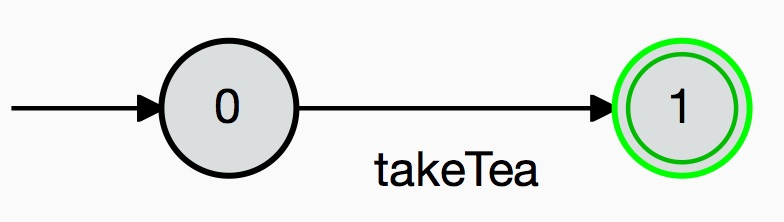
\includegraphics[scale=0.15]{Simple.jpg}\end{minipage}\hspace{\fill}

\noindent  Every process we define can be represented by a transition labeled automata. The events, like  \verb$takeTea$,  have an informal meaning (semantics) given by relating them to  some  real world event. We can prefix  a second event

\noindent\begin{center}  \begin{minipage}{0.45\textwidth}
\verb$Two = (teaButton->takeTea->STOP).$

\verb$Two = (teaButton->Simple).$   \end{minipage}\begin{minipage}{0.45\textwidth}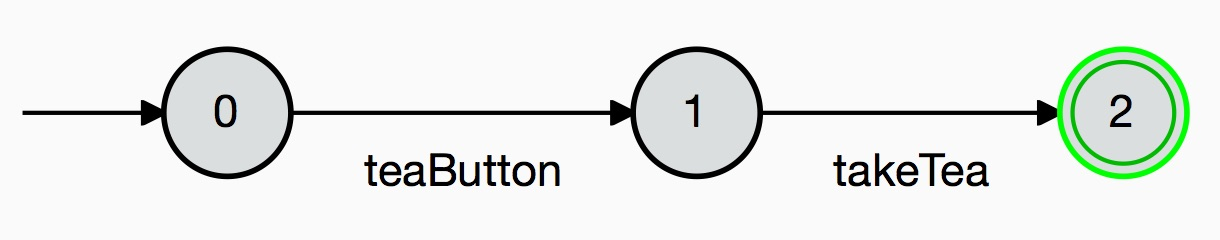
\includegraphics[scale=0.15]{Two.jpg}\end{minipage}\end{center}

The two definitions of \verb|Two| produce the same automata. If you only want to see \verb|Two| then you can suppress the production of the initial automata \verb|Simple| by add \verb|*| as a suffix to the name:

\noindent\begin{center}
\begin{minipage}{0.45\textwidth}\begin{verbatim}
automata {
  Simple* = (takeTea->STOP).
  Two = (teaButton->Simple).
}\end{verbatim} \end{minipage}
\end{center}

 The informal meaning of events  will  in part be formalised  by our  definition (to be given later) of  parallel composition. Informally we need to think of our events as \emph{hand-shake events}, i.e. event that can be blocked or enabled by the context in which they execute. For example the \verb$teaButton$ event of a vending machine can only occur when some agent actually pushes the button.  The pushing of the button  can also be modelled  by the \verb$teaButton$ event.



%\verb$$  \hspace{1em}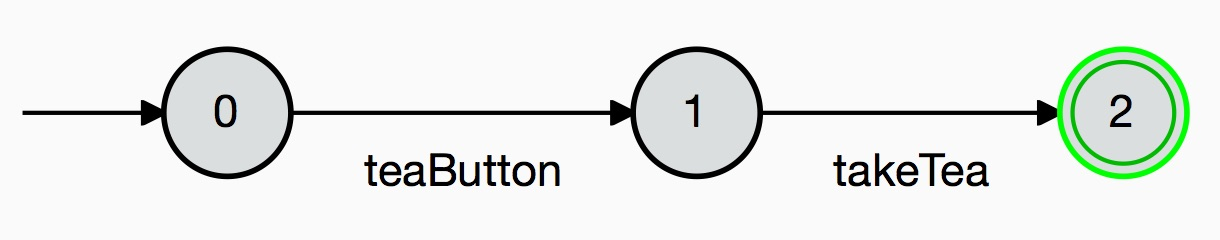
\includegraphics[scale=0.15]{Two.jpg} \end{center}

\subsection{Event choice}
A vending machine that has two buttons one for coffee the other for tea offers the user the \emph{choice} to push either button. We model this using the \emph{choice operator} \verb$_|_$.



\noindent\begin{center}  \verb$CM = (teaButton->takeTea->STOP|coffeeButton->takeCoffee->STOP).$

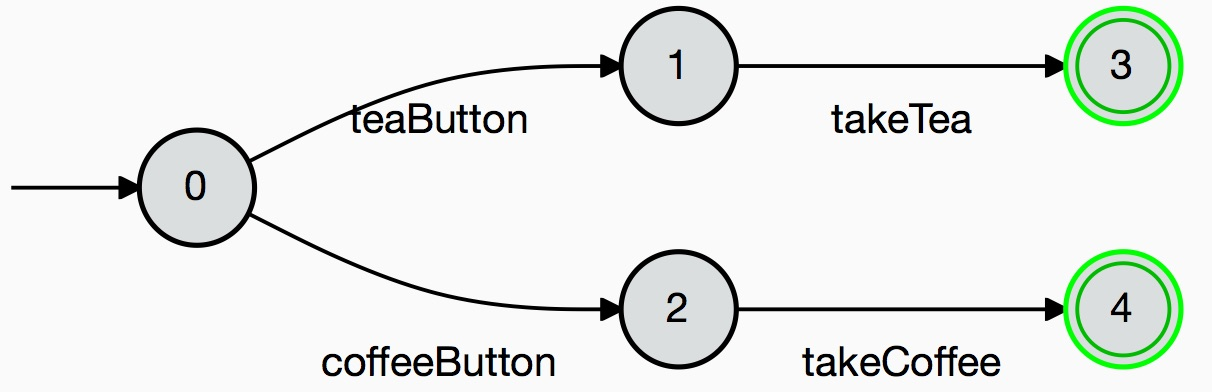
\includegraphics[scale=0.15]{CM.jpg}\end{center}

\noindent this automata {\bf \it branches} at the  initial node.

\subsubsection{Non deterministic processes} \label{sec:ndfa}
The two processes {\sf VM}  and {\sf VMx} both represent a vending machine that offers two drinks, {\sf tea} and {\sf coffee} after a coin is inserted. The two  terms are different and they are represented by  different automata.

\noindent\begin{center}
\begin{minipage}{0.8\textwidth}
\begin{center}\begin{verbatim}
automata
{
  VM = coin->((teaBtn->tea-> STOP)|(coffeeBtn->coffee->STOP)).
  Vmx = (coin->teaBtn->tea-> STOP)|(coin->coffeeBtn->coffee->STOP).
}
\end{verbatim}
%\end{minipage}
%\begin{minipage}{0.6\textwidth}
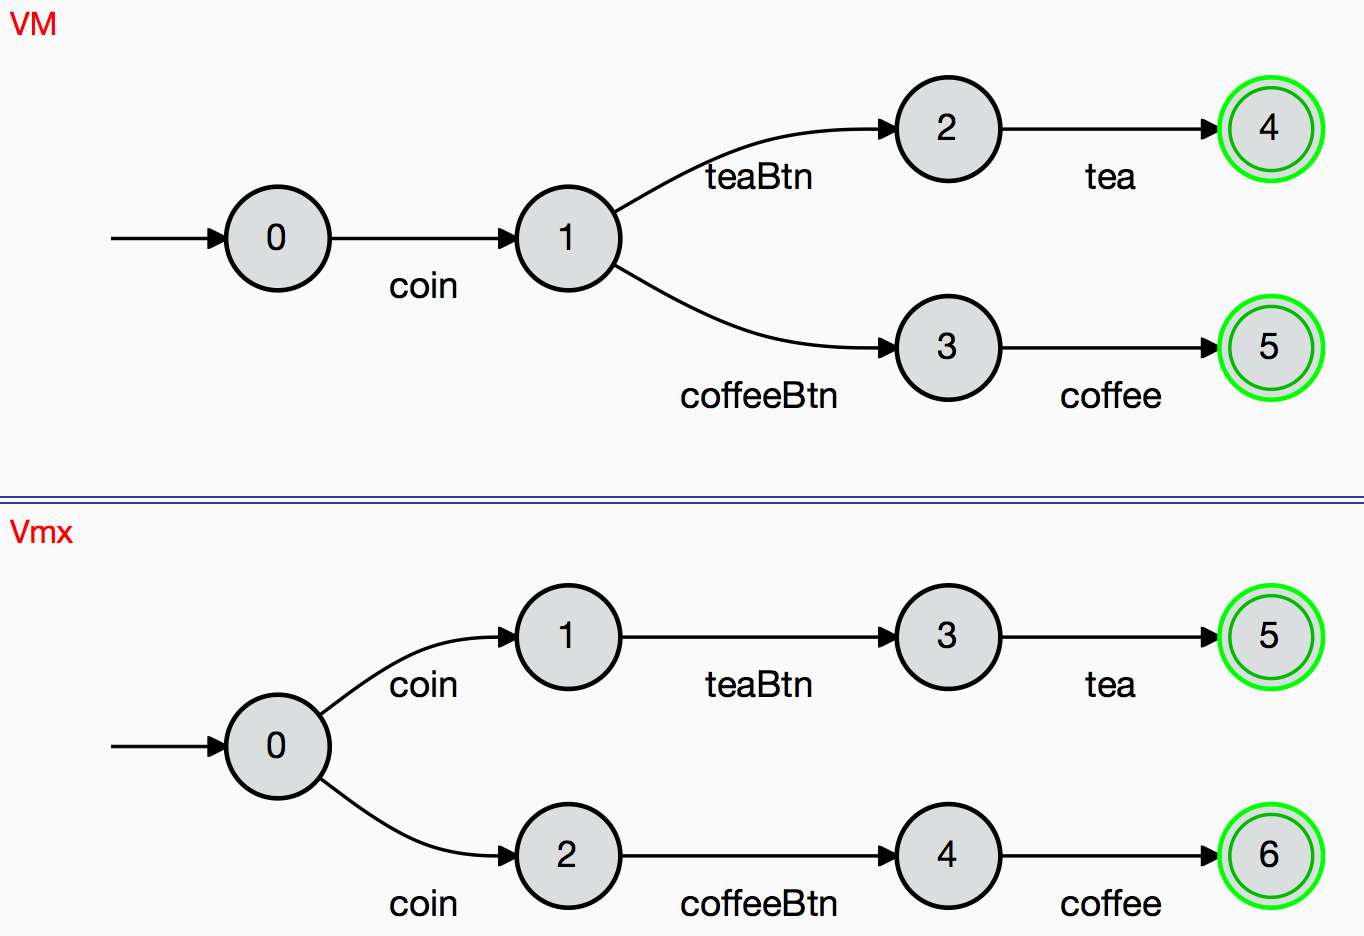
\includegraphics[scale=0.4]{ND.png}
\end{center}\end{minipage}

\end{center}

Are  {\sf VM}  and {\sf VMx}  equivalent processes?  Before you can answer this you must decide what  it means for two processes to be equivalent and there is many reasonable answers to this. If we assume either that the processes generate events or that they ae used to recognise a sequence of events then the processes can reasonable be viewed as equivalent as both generate (recognise) the same two event sequences:
\begin{enumerate}
\item \verb|coin,teaBtn,tea|
\item \verb|coin,coffeeBtn,coffee|
\end{enumerate}

But what if you were interacting with these processes and you wanted \verb|coffee| then  with the first machine you could always insert a \verb|coin| than push the \verb|coffeeBtn| and you would be able to get your \verb|coffee|. In contrast with the second machine after inserting the \verb|coin| you would not be able to push the \verb|coffBtn|. Hence you would be able to distinguish the two processes. It is this notion of indistinguishable by any test that we are interested in here.


\subsubsection{Properties of Choice}
 Choice is symmetric in that \verb$X|Y$ is equal to \verb$Y|X$. In what follows we write process equality as $\sim$ and hence:
 \[\sf X|Y\sim Y|X\qquad X|(Y|Z)\sim (X|Y)|Z\]
 details about, $\sim$,  process equality follow much later. 

The Choice between two identical processes is no real choice and hence:
\[\sf X|X\sim X\qquad X|STOP \sim X\]
Meaning has been  given to Processes in the form of an Axiomatic Algebraic semantics see \cite{BaW90}. Here we give meaning to processes by defining their operational behaviour as automata. From the details of what constitutes an automata we can see that the above equalities hold for our semantics. Looking at the same thing the other way in \cite{BaW90} they first define the algebraic properties of processes and then show the automata satisfy them.

{
\subsection{Internal  Choice $+$}
Defined in CSP and ATP but not in ACP nor CCS.
Used to represent a process that internally, with no external involvement, can choose to behave like either process. Consequently such a process can not be guaranteed to behave like either of the processes.

The relation between the two definitions of choice is captured by the axioms:


\[\sf (a->A+a->B) =_F (a->A|a->B) =_F (a->(A+B))\]

{\color{red} NOT bisim need to use testing or Failure equality!}

Internal choice is best modelled by allowing automata to have a set of start states. Using a set of start states  facilitates the modelling of processes  with either  probabilistic choice or  \emph{active} actions.

\subsubsection{Properties of Internal Choice}
 Choice is symmetric in that \verb$X+Y$ is equal to \verb$Y|X$. In what follows we write process equality as $\sim$ and hence:
 \[\sf X+Y\sim Y+X \qquad X+(Y+Z)\sim (X+Y)+Z\]
 
 

}
\subsection{Sequential composition}

Two processes can be composed in sequence using \verb|=>|   and sequential composition satisfies:

\[\sf ((a->STOP)=>A) \sim (a->A),\qquad
X=>(Y=>Z) \sim (X=>Y)=>Z\]

\[\sf (STOP=>A) \sim A, \qquad (A=>STOP) \sim A \]

\[\sf (X|Y)=>Z \sim (X=>Z)| (Y=>Z), \qquad 
(X+Y)=>Z \sim (X=>Z)+ (Y=>Z)\] 

\[\sf W=>(X+Y) \sim (W=>X)+ (W=>Y) \sim (W=>X)| (W=>Y)\]





\subsection{Non terminating processes}
We call the set of know  processes  the  \emph{Process name space}.   Initially the  \emph{Process name space} is \verb${STOP}$.    Each process definition \verb$P1 = ...$ adds the the defined process \verb$P1$ to the name space.

Processes consist of a set of states, an initial state  and a set of event labelled state transitions. Given  a process has a set of states and a set of transitions it is reasonable that the process can be \emph{conceptual identified} with its initial state.


Clearly any state \verb$S$ in process \verb|P1| could also  be \emph{conceptual identified}  with the the process consisting of the same set of states and transitions but with initial state \verb$S$.  We use this idea to define non terminating processes.  By allowing any valid process to be used where \verb${STOP}$ has been used we can define non terminating or cyclic processes.


To build events that do not terminate we can replace \verb$STOP$ with the name of the process we are defining thus \verb$T = (takeTea->STOP).$ becomes \verb$Tt = (takeTea->Tt).$  The  process \verb$Tt$ can endlessly perform the \verb$takeTea$ event.

\noindent
\begin{minipage}{0.45\textwidth}\begin{center}
\verb$Tt = (takeTea->Tt).$

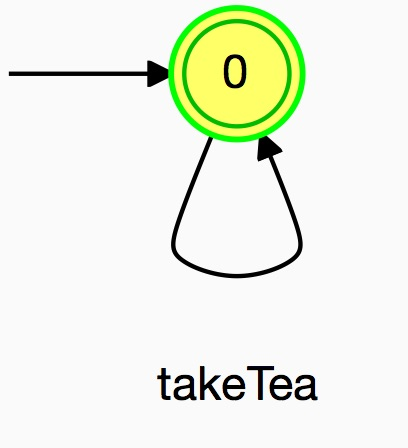
\includegraphics[scale=0.15]{Tt.jpg} \end{center}\end{minipage}
\begin{minipage}{0.45\textwidth}
\begin{center}
\verb$BT = (teaButton->takeTea->BT).$

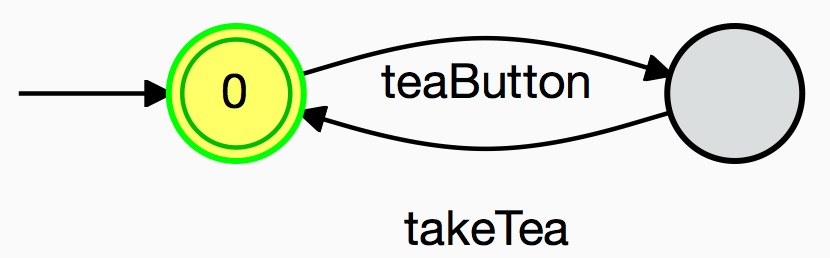
\includegraphics[scale=0.15]{BT.jpg}\end{center} \end{minipage}

  We allow \emph{local process} or states to be defined within a process  definition by separating definitions with a comma. The local process do not appear in the Process name space.

\begin{center}\begin{minipage}{0.25\textwidth}
\begin{verbatim}
P = (a->Q ),
  Q = (b->P|c->Q).
\end{verbatim}
\end{minipage}
\begin{minipage}{0.25\textwidth}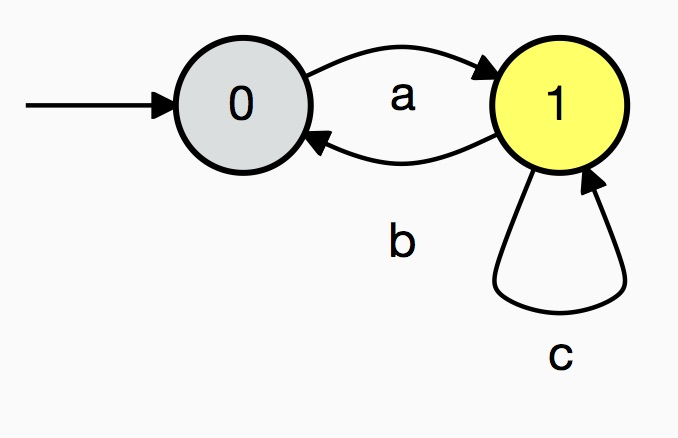
\includegraphics[scale=0.15]{P.jpg}
\end{minipage}
\end{center}
This allows complex processes to be defined without cluttering the \emph{Process name space}.

\subsection{Translating any finite state automata  into a process term}
It is often easy to   sketch  your understanding of a processes behaviour as an automata. Then from any automata  we can construct  the  process term with  the behaviour given by the automata.  Our tool  will automatically generate  the automata from the term.  The generation of the term from the automata  can be achieved quite mechanically as follows:

\begin{enumerate}
\item name all nodes (or all nodes with more than one in and one out event) with a process name
\item define each of the processes and the choice of events leaving them
\item end each process definition with a comma except for the last process that must end with a full stop.
\end{enumerate}

\noindent\begin{center} 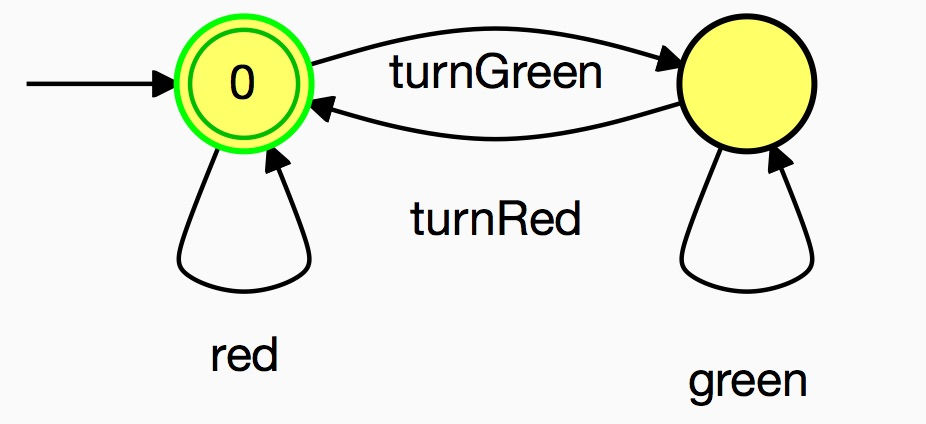
\includegraphics[scale=0.15]{TrRed.jpg} \end{center}

For the above automata node {\sf 0} we name \verb$TrRed$ and  node {\sf 1} we name \verb$TrGreen$. Then we define the events leaving these nodes
\begin{center}\begin{minipage}{0.5\textwidth}
\begin{verbatim}
TrRed = (red->TrRed | turnGreen ->TrGreen),
  TrGreen = (green->TrGreen|turnRed->TrRed).
\end{verbatim}
\end{minipage}\end{center}

  The result of this construction is the definition of the first process \verb$TrRed$, all other processes, in this case just  \verb$TrGreen$, are  {\bf \it local} definitions.

\section{Semantics of processes with atomic events}
 Distinct automata can be used to  represent exactly the same process. We formalise this be defining a semantic equivalence  of automata.  The question as to what automata should be equated and how do you justify you notion of equality we leave to later. Here we are going to introduce to very different notions of process equality that are widely used and widely discussed in the literature.




 \subsection{Complete Trace equality}\label{sec:Trc}
 The trace semantics of a process are the set of executions the process can undertake.

 Complete finite traces must end in state from which not event can occur:
 \[Tr_{Fin}({\sf P}) \triangleq \{ tr : \exists n : \aro{S_{\sf P} }{tr}{n}\land \pi(n)=\emptyset\}\]

 Infinite traces  do not end:
 \[Tr_{Inf}({\sf P}) \triangleq \{ tr :  \aro{S_{\sf P} }{tr}{}\}\]

 The  complete traces of a process

 \[Tr_c \triangleq Tr_{Fin}\cup Tr_{inf}\]

 Complete trace equality:

 \[{\sf P} =_{Tr_c} {\sf Q} \triangleq Tr_c({\sf P}) = Tr_c({\sf Q})\]

Trace equality dose not distinguish deterministic processes from non deterministic processes  and hence the two processes in \sref{ndfa} are identified.
 \subsection{Bisimulation}\label{sec:biscol}
  A bisimulation  $\sim$ is relation on the nodes of an automata  that is  symmetric  $n\sim m\Rightarrow m\sim n$  and

 \[ n\sim m \land \aro{n}{a}{n'}\Rightarrow \exists m' . \aro{m}{a}{m'} \land n'\sim m' \]

 Two processes {\sf P} and {\sf Q} are bisimular if and only if there is a bisimultaion relation that relate their start nodes, ${\sf P_S\sim Q_S}$.

 Bisimulation equivalence is much finer than complete trace equality and  only equate processes that could not possibly be distinguished.
 Consequently the two processes in \sref{ndfa} are not bisimular (bisimulation equivalent).

 To help us understand how bisimulation equivalence works we give a simple co-inductive algorithm to compute the maximal  bisimulation relation  using a node colouring where  nodes with the same colour  are related.

\begin{center}\begin{minipage}{0.7\textwidth}

 {\bf 1.} Initially colour all nodes with the same colour.

{\bf 2.} Repeatedly recolour the nodes using
     \begin{center}
     $Col_{i+1}(n) \triangleq \{(a,Col_i(m)) .\aro{n}{a}{m}\}$
     \end{center}

{\bf 3.} \hspace{0.25in} stop when  the recolouring changes nothing.
\begin{center}
     $Col_{i+1}(n) =Col_{i+1}(m) \Leftrightarrow Col_{i}(n) =Col_{i}(m)$
     \end{center}

\end{minipage} \end{center}

 The maximal bisimulation relation that  can be computed very quickly and  bisimular nodes, nodes with the same colour, can be identified to produce a simpler automata. .
 Using this colouring algorithm it is easy to see the result of applying  bisimulation simplification to simple automata.

 This algorithm can be applied to many automata at the same time and can be used to compute an equivalence   class on a set of   automata.
 Bisimulation has  attractive mathematical properties, is easy to compute and has proven to be of practical use. Consequently bisimulation relations have been defined on many different structures.

Both these equivalences are congruent with respect to our process operators (substitution of equivalent processes).
\[ A\sim B \Rightarrow A||P\sim A||P\]
\[ A =_{Tr_{c}}  B  \Rightarrow  A||P =_{Tr_{c}}  A||P\]

\section{Event hiding and process simplification}
Our process language can be used both to specify \emph{implementations}  of  processes and more abstract \emph{specifications}.  Our tool is designed to support the approach popularised by Event B. Both the abstract specification and the more concrete implementation are specified in the same language.  The tool then checks that the implementation is a \emph{refinement} of the specification.

In our event based approach events in the implementation but not the specification are hidden by abstraction and the resultant process is checked for equality with the specification.  In this section we define event hiding and abstraction.



We can make events private  by  hiding them so they can not be seen.  \verb|_\{t}| operator renames the {\sf t} event to the unobservable  {\sf tau} event.

See following example:

\begin{minipage}{0.45\textwidth}
\noindent\begin{center}\verb$Basic = (a->(t->b->STOP | c->STOP))\{t}.$

 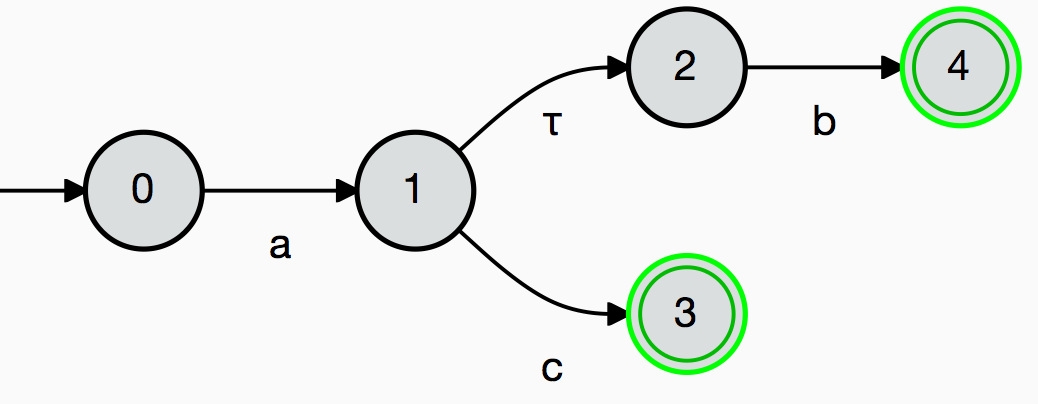
\includegraphics[scale=0.4]{BasicTau.png}
 \end{center}
 \end{minipage}\hspace{\fill}
\begin{minipage}{0.45\textwidth}
\noindent\begin{center}
\verb$B = abs(Basic).$
 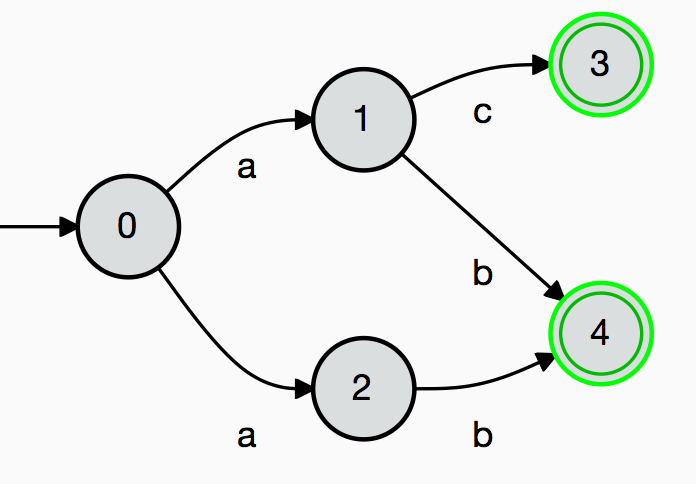
\includegraphics[scale=0.6]{Basic.png}
 \end{center}
 \end{minipage}

 In the above example \verb|abs| introduces two observable events:
\begin{center}
 \begin{minipage}{0.7\textwidth}
 \begin{enumerate}
 \item ${\sf \aro{0}{a}{2}}$  in place of  the event sequence ${\sf \aro{0}{a}{1}}$  and  ${\sf \aro{1}{\tau}{2}} $
 \item ${\sf \aro{1}{b}{4}}$  in place of  the event sequence ${\sf \aro{1}{\tau}{2}}$  and  ${\sf \aro{2}{b}{4}} $
 \end{enumerate}
   \end{minipage}
 \end{center}


 The \verb|abs(_)|  operator abstract away the {\sf tau} events. To cope with cases where many $\tau$ events can be executed one after the other we first define  $\Aro{x}{\tau}{y}$.

  A sequence of zero or more $\tau$ events
  \[\Aro{x}{\tau}{y} \triangleq \exists i\geq 0 : \exists n_1,n_2,..n_i :\aro{x}{\tau}{n_1}, \aro{n_1}{\tau}{n_2}\ldots \aro{n_i}{\tau}{y}\]
   can be  executed unseen and are represented as $\Aro{x}{\tau}{y}$. When $i=0$ we have $\Aro{x}{\tau}{x}$ for any $x$.


 Abstraction constructs, $\Aro{x}{\sf a}{y}$ the observable semantics:


   \[\Aro{x}{\sf a}{y}  \triangleq \exists u,v :   \Aro{x}{\sf \tau}{u} \land  \aro{u}{\sf a}{v}  \land \Aro{v}{\sf \tau}{y}
 \]


 \subsection{Event hiding and non terminating processes }

 The literature is divided on how to hide $\tau$ events that loop.  CSP  refers to these processes with $\tau$ loops  as \emph{diverging} and models them as having potentially \emph{chaotic} behaviour. CCS   and Discrete Event Systems DES, assumes them to be benign as simply prunes them. Here we offer both options. The CSP option assumes that the system can behave \emph{unfairly} and the CCS option assumes the system behaves \emph{fairly}.



 The command \verb|abs(_)| is based on the fair assumption and \verb|abs{unfair}(_)| is based on the unfair assumption.



With the unfair assumption congruence with respect to interleaving parallel composition requires some care because the relation  between events from parallel components is \emph{fair}. That is to say the infinite execution of an event from on process can not prevent the parallel process executing an unrelated event.

In other words one process, {\sf P},  diverging will not effect the events of a second process, {\sf Q},  running in parallel whereas with the unfair assumption it can block other events on {\sf P}. But with interleaving composition ${\sf P\parallel Q}$ the events of {\sf P} and {\sf Q} can no longer be distinguished.

To accommodate this label nodes on a $\tau$ loop as divergent and require that parallel composition preserves divergence. This has the effect of allowing divergence of {\sf P} to block the events of {\sf Q}.

{\color{red} bug to be checked}
\noindent\begin{center}
\begin{minipage}{0.3\textwidth}
\begin{verbatim}
automata {
S* = a->X,
   X = (t->X|b->STOP).
Simple = S\{t}.
O* = Simple||(d->STOP).
One = abs{unfair}(O).
T* = abs{unfair}(Simple).
Two = T||(d->STOP).
}
\end{verbatim}\end{minipage}
\begin{minipage}{0.5\textwidth}
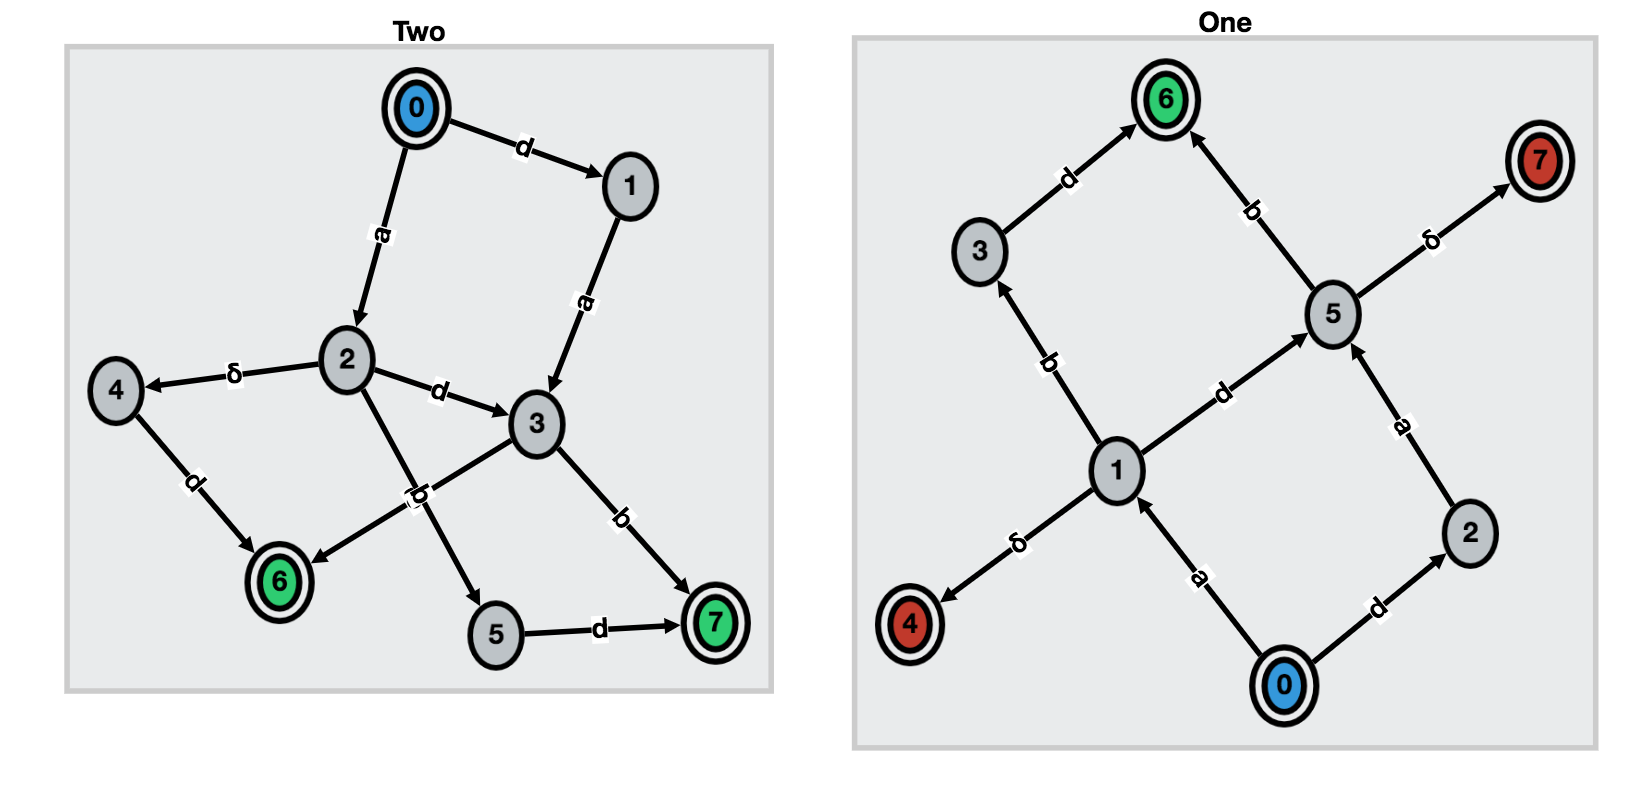
\includegraphics[scale=0.3]{OneTwo.png}
\end{minipage}\end{center}
Pragmatically divergence and deadlock are rarely wanted and their existence merely indicate that the definitions are erroneous. In such situations it is unimportant how we model divergence as it will be removed. In situations where we do want to model process with deadlock  or divergent behaviour then we need to be more careful.


Frequently we are interested in how a system behaves when errors occur but when errors occur is rarely determined exactly. Hence modelling a systems correct and error behaviour will introduce some probabilistic or non deterministic behaviour. Hiding both errors and their handling may introduce divergence and this may be best interpreted \emph{fairly}.


\section{Concurrent Processes }
So far we have have defined sequential processes but now we wish to define how two sequential processes behave when they are both run together. This is modelled using the parallel composition operator $\_\parallel\_$.
Two processes run in parallel can only interact via event synchronisation How this is defined depends upon the interpretation you wish to give your events. In what follows we consider two distinct styles of events, hand shake events as found in CSP and CCS as well as broadcast events as found in IOA.

\subsection{Handshake synchronisation }

Two processes run in parallel can only interact via event synchronisation and events on only synchronise with other event having the same name.

Below we have two processes each with three events and no two event have the same name hence the event from each process can be {\bf interleaved} in any way.

 \begin{center}
 % \fbox{
\begin{minipage}{0.4\textwidth}
\begin{verbatim}
P = ((a->b->c->STOP) || (x->y->z->STOP)).
\end{verbatim}
\end{minipage}
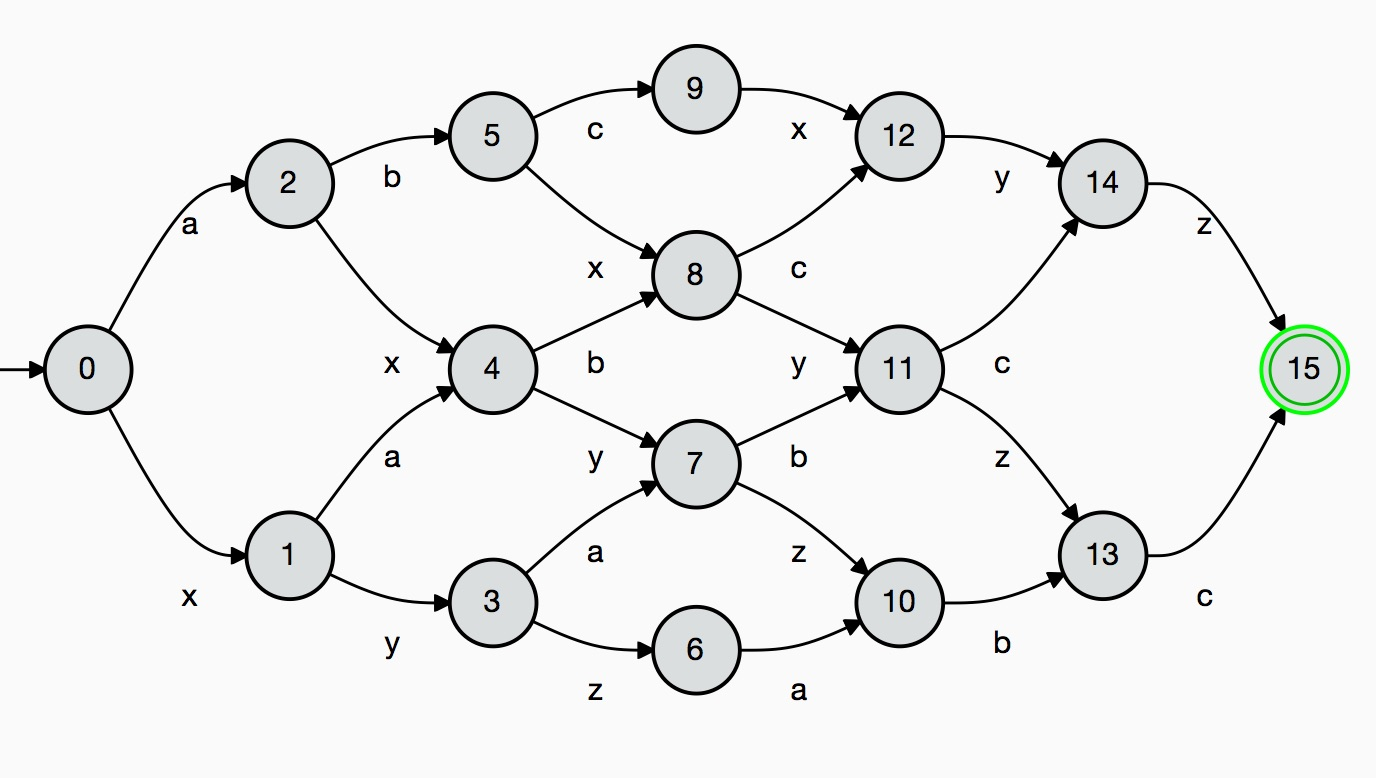
\includegraphics[scale=0.2]{par.jpg}
\end{center}
This definition of parallel composition equates parallel processes with a single sequential process. As such some aspects  of real parallel processes are lost. Some times this  equality is referred to as being based upon the \emph{interleaving assumption}.



Without synchronization  two processes   are independent and hence their events interleave and the state space of the composition of the processes is the product of the state space of the constituent processes.


   In the Process tool events from different concurrent processes that have the same name must synchronize and only these events synchronize. That is neither process can  execute the synchronising event on its own.  These  synchronising events are only executed when both processes are ready to execute them.
  Below only differs  from the previous process in that the second event in both processes has the same name and hence must  synchronize and the resulting \verb$m$ event is then hidden (renamed $\tau$).


 \begin{center}
\begin{minipage}{0.5\textwidth}
\begin{verbatim}
P = ((a->m->c->STOP) || (x->m->z->STOP))\{m}.
\end{verbatim}
\end{minipage}

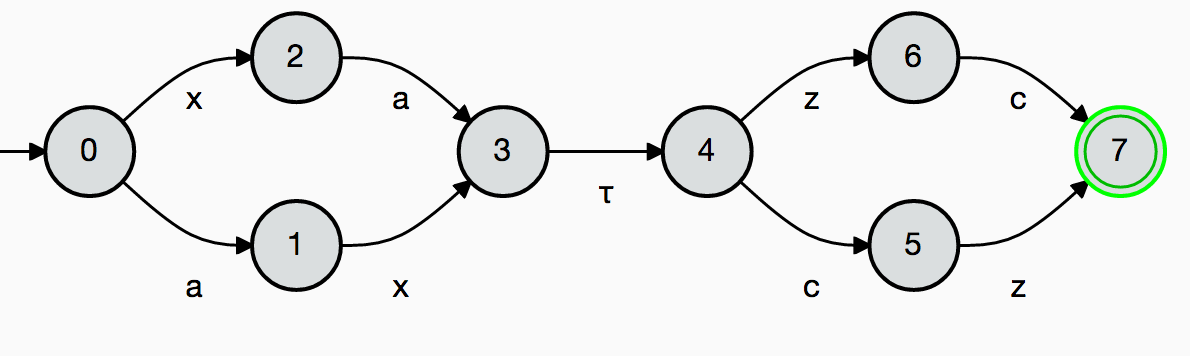
\includegraphics[scale=0.5]{Sync.png}

\end{center}

\noindent Event synchronization is the only mechanism for concurrent process interaction and because of event synchronisation we know:

\begin{quote}
{\bf If you can see and event you can synchronize with it and you can block it.}
\end{quote}





 Hence the only way  the  control the order of two events from different concurrent   processes is to introduce a synchronizing event. In above the \verb$a$ event and the \verb$z$ event are from different concurrent processes in the interleaving example either could occur first. Whereas in the synchronization of the \verb$m$ events forces the \verb$a$ event to occur before the \verb$z$.

Another  effect of synchronization   is to reduce the size of the reachable state space of the automata. Note the first two events {\bf a} and {\bf x} can be performed in either order but only when both {\bf a} and {\bf x} have been performed and both processes are ready to perform {\bf b} dose the {\bf b}  event actually get performed.


\subsection{Broadcast event synchronisation}
In the previous section when events from two processes synchronised  the the synchronising events from both processes were treated the same, both could block the other process. This style of synchronisation captures real events such as {\sf pushing a button} I cannot push a button that is not there or is frozen nor can  button on a vending machine be pushed if  I am not prepared  to push it. Both me and the vending machine must wait for the other to be ready before the {\sf buttonPush} event can occur.


\begin{center}\verb$(a -> broadcast! -> c -> STOP)||(x -> broadcast? -> y -> STOP)$

	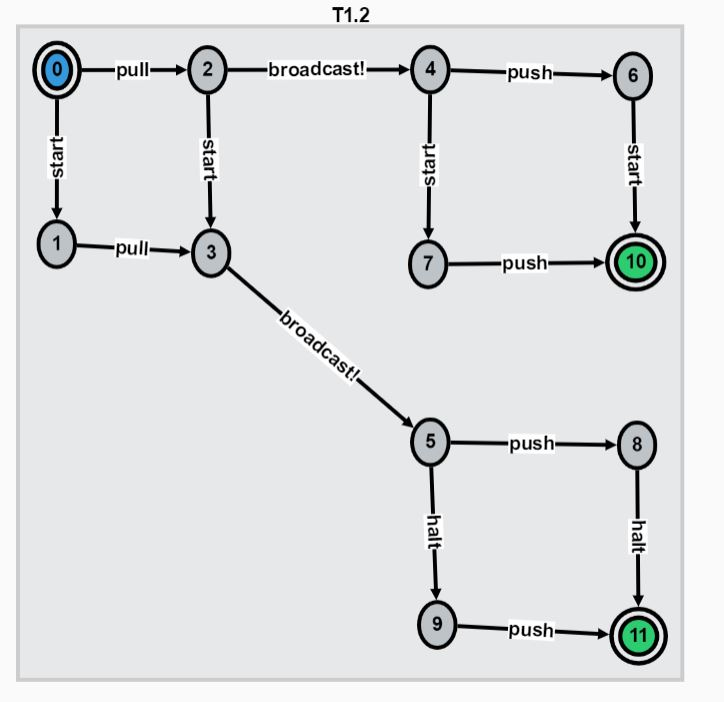
\includegraphics[scale=0.5]{bcast.jpg} \end{center}




Other events are not like a {\sf broadcast!}  events cannot be blocked by a process not being ready for them. Real examples include:  I can send an email even if you are not ready to read it. A traffic light  is green even if no one is observing it.  Such interactions  by defined with  \emph{\bf unblocking send} events and \emph{receive} events.

\hspace{\fill}
\begin{tabular}{ll}
send radio warning & {\sf warning!} \\
hear radio warning & {\sf warning?}
\end{tabular} \hspace{\fill}
\begin{tabular}{ll}
green light is shining  & {\sf green!} \\
I see the green light & {\sf green?}
\end{tabular}
\hspace{\fill}



Non-blocking send events can be decomposed into:
\begin{description}
\item[point to point] Emails are often messages from one person to one other  unique person.
\item[multicast] A traffic light can be seen by many cars.
\end{description}

The point to point interaction can  defined with: 



\begin{center}\verb$(start -> broadcast! -> halt -> STOP)||(pull -> broadcast? -> push -> STOP)$
\end{center}
The automata  can be seen  below:
\begin{center}	
	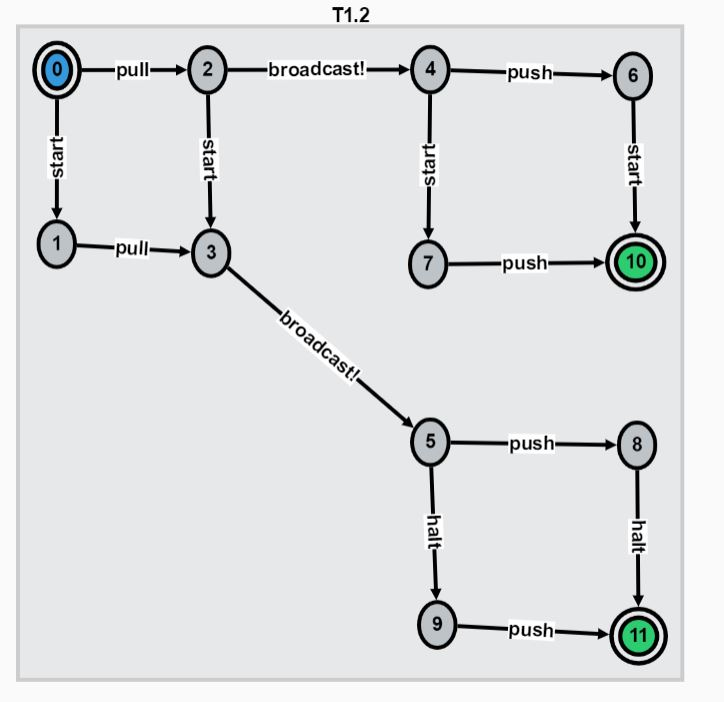
\includegraphics[scale=0.5]{bcast.jpg} \end{center}
	
	
	
Note: if you are not listening you might miss the warning and if you are not looking you might not see the green light. Listening/looking is formalised as being in a state from which the receive event is enabled. We model processes so that if you are listening/looking then you will hear/see the broadcast event.



Considering systems containing separate processes for  {\sf Cars} and {\sf Traffic Lights} we often need to consider the case when the {\sf Traffic Lights} are unique but there are many {\sf Cars}.  The {\sf Cars} do not interact but if two cars are both looking then they will both see the green light when it is on.

Consequently wo  {\sf braodcast?} events will not synchronise  like  hand shake events but behave as shown below:




\section{ Renaming events and simplifying Processes}
Frequently when we are thinking of one process it is natural to give an event a particular name. But, when considered from the perspective of another process that may interact with it this name might be confusing. Consequently we introduce ways to rename events.
Finally we show how bisimulation colouring can be used to simplify processes. To aid understanding we will consider a simple buffer example in the following.
\subsection{Labelling Processes}
In the following example we make use of a one place buffer \verb$Buf$ is a process that when empty can receive some thing \verb$in$ and when full can return it \verb$out$.
\noindent\begin{center} 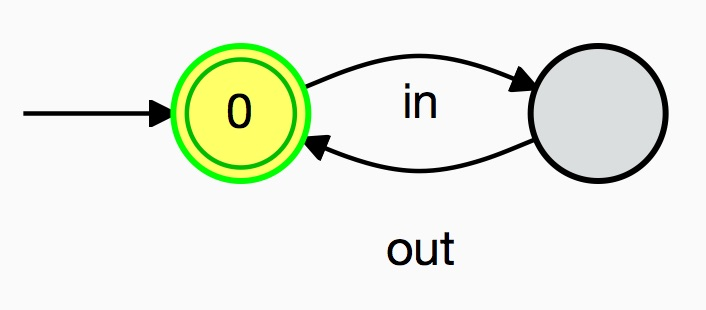
\includegraphics[scale=0.15]{Buf.jpg} \end{center}
By labelling  processes  \verb$one:Buf$ the tool  labels all events in the process \verb$one.in$ and \verb$one.out$.

Using process labelling we can make two differently label copies of a process and compose them in parallel to build the interleaving of the two copies.


\noindent\begin{center}\verb$B2=(one:Buf||two:Buf).$\end{center}

\noindent\begin{center} 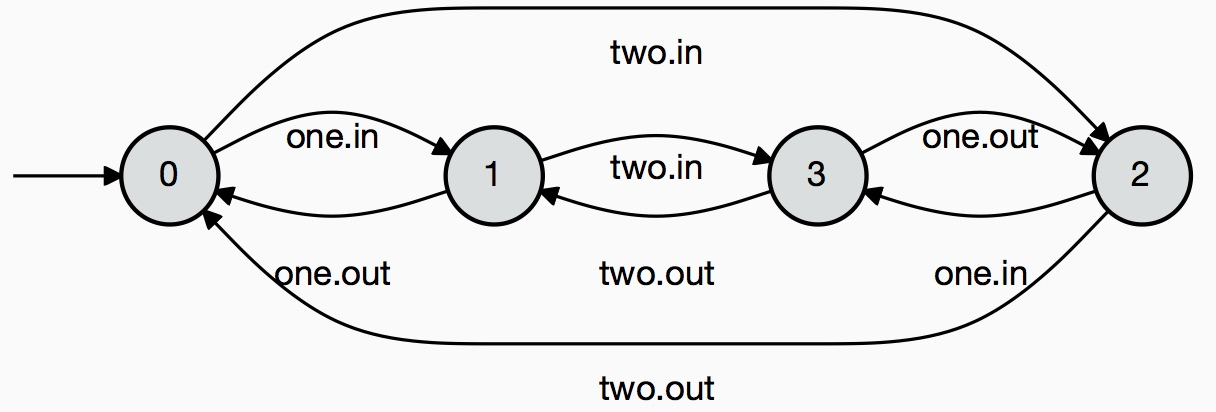
\includegraphics[scale=0.15]{B2.jpg} \end{center}


\subsection{Event renaming}
If two events from processes run in parallel have the same name they, and only they,  must synchronise.
\begin{quote}
{\bf Pragmatically when you compose two processes in parallel you should check the name of events   you want to   synchronise and where necessary rename them to enforce the desired synchronisation.}
\end{quote}


We force the synchronisation of the output from buffer \verb$one$ with the input to buffer \verb$two$ by event renaming.


\noindent\begin{center}\verb$B3 = (one:Buf/{move/one.out}||two:Buf/{move/two.in}).$\end{center}

\noindent\begin{center} 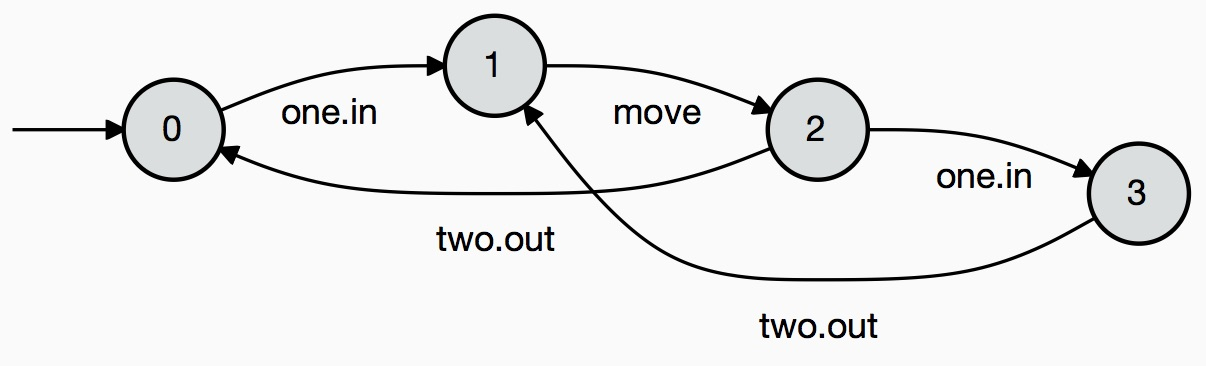
\includegraphics[scale=0.15]{B3.jpg} \end{center}

Note that the result is much simpler than the interleaving as the \verb$move$ event now can only occur when {\bf both} buffers are able to perform it.



\subsection{Process simplification}
We can go further and hide the \verb$move$ event  by applying \verb$_\{move}$ The \verb$move$ event  becomes a \verb$tau$ event that can neither  be synchronized with nor blocked.

\begin{minipage}{0.45\textwidth}
\noindent\begin{center}\verb$B4 = B3\{move}.$

 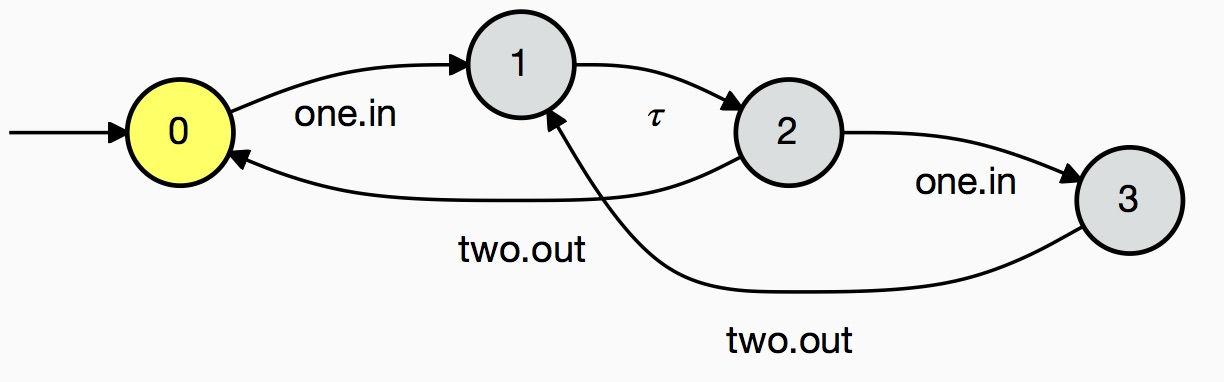
\includegraphics[scale=0.15]{B4.jpg} \end{center}
 \end{minipage}
\begin{minipage}{0.45\textwidth}
\noindent\begin{center}\verb$B5 = abs(B3\{move}).$

 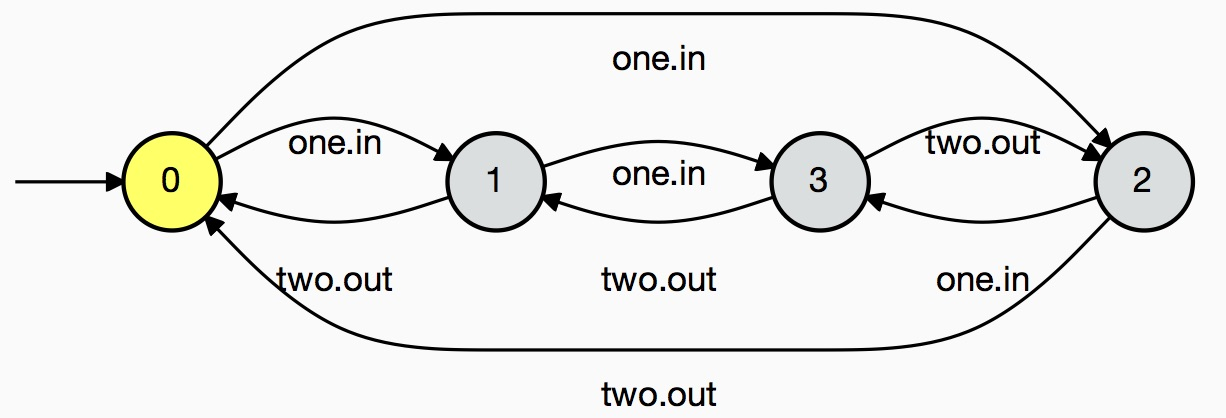
\includegraphics[scale=0.15]{B5.jpg} \end{center}
 \end{minipage}

The \verb$tau$ events  can be removed by {\bf abstraction}, (the application of \verb$abs(_)$) otherwise known as building the \emph{observational} semantics.  With a little effort nodes, 1 and 2 in \verb$B5$ can be seen to be  essentially the same.  They are actually bisimular but we will not be going into details here. These nodes can be identified to produce a simpler but equivalent automata by the application of \verb$simp(_)$.



\noindent\begin{center}\verb$B6 = simp(abs(B3\{move})).$

 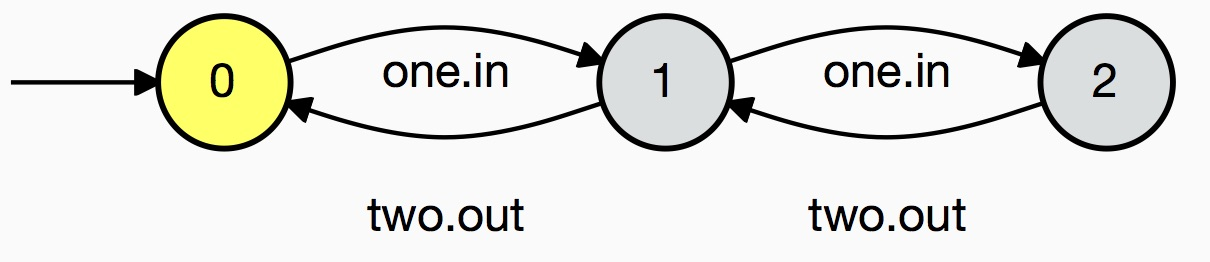
\includegraphics[scale=0.15]{B6.jpg} \end{center}


Event hiding is commonly, but not exclusively,   used to model private  communication.

\section{Testing and equality}
In this section we are going to introduce  a very generic notion of equality, testing equality. This can be applied to to any set of things all they need is an operator to compose them and a definition of how to observer them, here the set of things is our set of processes, the operator to compose then is parallel composition and finally when we observer a process all we can see is the complete trace of events that are executed.

When a non-deterministic system is tested it is placed in some context and the combination of the system and text context is executed, but this test must be run a number of times and the set of observations (results) recorded.
%Later when probabilistic systems are tested all we change is that in place of recording the set of observations what is recorded is the frequency with which the observations are made.


Our processes, {\sf E},  are taken from a set of processes $\Emath$. A context, ${\sf \_\parallel X}$, consists of a process, ${\sf X}\in \Emath$,  run in parallel with the process under test. Let  $\Xi\triangleq \{\_\parallel X | X\in \Emath\}$ be  the set of all contexts.
Placing  {\sf E} in context {\sf X} can be   written as  $[{\sf E}]_{\sf X}$ or as ${\sf X\parallel E}$.   A single experiment consists of observing a single execution of $[{\sf E}]_{\sf X}$ and  results in a single trace, taken from a set of possible observations $Tr^c$, being recorded.
For non deterministic processes the experiment must be repeated and a set of observations $Tr^c$, being recorded.

A specification can be  interpreted as a \emph{contract} consisting of the \emph{assumption} that the process will be placed only in one of the specified contexts $\Xi$ and a \emph{guarantee} that the observation of its behaviour will be one of the observations defined by the mapping $O: \Emath \rightarrow\Xi\rightarrow \wp Tr^c$.  The mapping $O$ defines what can be observed  for all processes in any of the assumed contexts. Hence for any fixed $\Xi$  we have a definition of the semantic equivalence of processes.

\emph{Definition}

%Let $\Xi$ be a set of contexts each of which the processes ${\sf A}, {\sf C} \in \Emath$ can communicate privately with, and let $O: \Emath \rightarrow\Xi\rightarrow \wp \Obsmath$ be a function which returns a set of observations, \ie\ a subset of $Tr^c$. Then, the relational semantics of a process ${\sf A}$ is a subset of $\Xi \times Tr^c$.
\[
 \llbracket {\sf A}\rrbracket_{\Xi,O} \triangleq  \{(x,o) | x \in \Xi \wedge  o\in O([{\sf  A}]_x)\}
\]
%and refinement is given by
%\[
%{\sf A} \sqsubseteq_{\Xi, O} {\sf  C} \triangleq   \llbracket {\sf C}\rrbracket_{\Xi,O} \subseteq  \llbracket {\sf A}\rrbracket_{\Xi,O}
%\]
and equality is
\[
{\sf A} =_{\Xi, O} {\sf  C} \triangleq   \llbracket {\sf C}\rrbracket_{\Xi,O} = \llbracket {\sf A}\rrbracket_{\Xi,O}
\]
%\footnote{The definitions in this section are taken from \cite{ReS09} where they have been applied to both state-based and event-based models.}

Let $\Emath$ be the set of LTS and $Tr^c$ be the complete traces of an automata  then all we need to define to fix our definition of testing equality is the definition of $\parallel$ parallel composition.
\hspace{\fill}$\Box$

In what follows we will define parallel composition between handshake events  and  another definition of parallel composition for broadcast events.  Using parallel composition for \emph{handshake events} the above definition of testing equality has been shown to be the same as the well known \emph{Failure equality} from CSP.  Whereas using parallel composition between \emph{broadcast events} the above definition of testing equality corresponds to the well known \emph{quiescent trace} equality.


\section{Indexed Process definitions}


Basic process definitions you have seen so far a fixed finite set of states. This accurately reflects  many situations very well and allows easy and complete push button verification. Alternatively when what you are modelling has infinite state or an unknown state size you could use symbolic models but verification  frequently requires  input from a domain expert and is very time consuming.

The approach adopted here is to define both states and events using an index and limit the size of the index by a parameter.  Prior to using a parameter it must be declared and given a fixed value. A finite state approximation of indexed process can be built and size of the approximation can be changed by changing the declared value of the parameter.

\subsection{The small world assumption}

Most program bugs can be found while restricting variables to range over a small domain. Using this assumption we  model processes with variables by indexing the processes and restricting the indexes to range over a small domain. Having done this the variables in the state can be removed by instantiating the variables with values from the small domain.

More than one parameter can be used to define a process.  Once all the parameters are fixed you are back to a basic process with a finite set of states and events.
Processes can be indexed in different ways to achieve  conceptually different things. The first we consider is how to build a process of parametrised    size,  the second is to model events that input or output data and finally how to model a parametrised number of concurrent processes.

\subsection{State indexing}

We can define a process consisting of an  an unknown number of states. To do this we must index the local states (or local processes).
We will consider a simple \verb|Purse| that can contain a number of \verb|coin|s. We define the \verb|Purse| based on a parameter \verb|N| that depicts its size.
\noindent\begin{center}
Automata for a \verb|Purse| that can contain 3 coins.

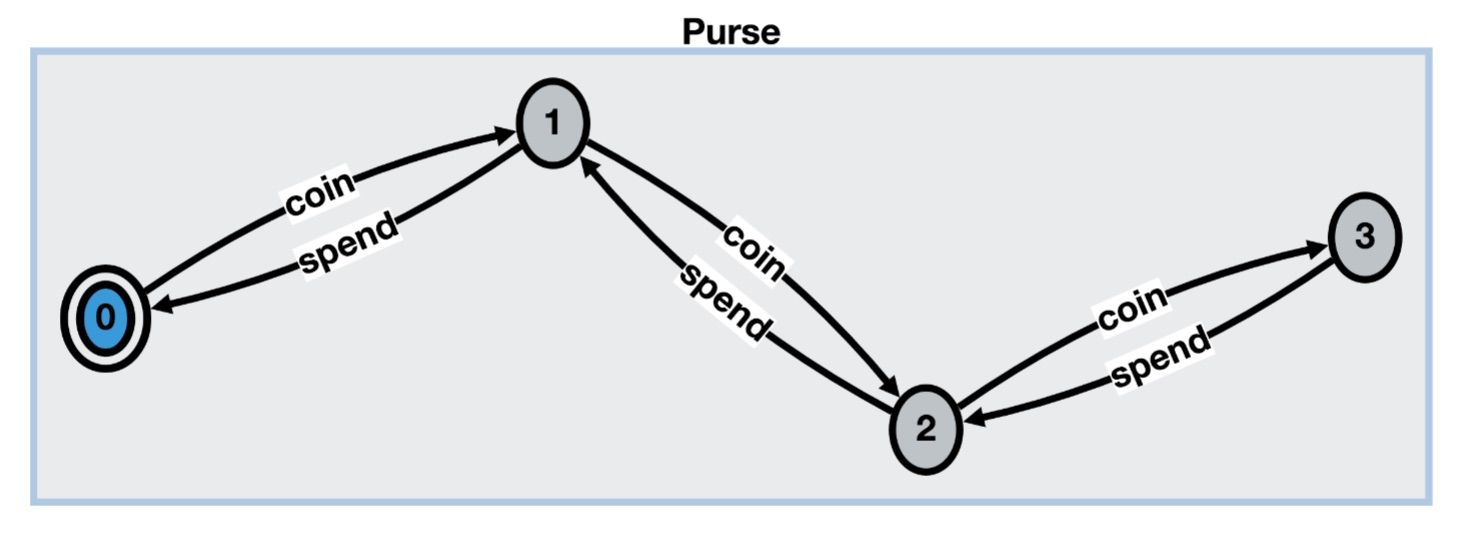
\includegraphics[scale=0.15]{Purse.jpg} \end{center}


The first thing we do is define a constant to be used for the size of the automata to be constructed:

\hspace{0.5in}\verb$const N = 3$

Next  we define the automata:

\begin{center}\begin{minipage}{0.5\textwidth}
\begin{verbatim}
automata {
Purse = P[0],
 P[c:0..N] = (when c<N  coin -> P[c+1] |
             when c>0  spend -> P[c-1]).
}\end{verbatim}
\end{minipage}\end{center}

The first line \verb|Purse = P[0],| defines that the purse is initially empty then  the definition \verb$P[c:1..N] =$    defines the \verb$N$ processes \verb$P[1],P[2]$ and \verb$P[3]$


The term \verb$P[c:1..N]$ on the left of the equality can be thought of  as assigning a value to a variable \verb$c$. The term \verb$P[c+1]$  on the right of the equality reads the value in the variable and then  "returns" to the purse in a new state where "c:=c+1".

On the right hand side of the equality we define guarded events:
\begin{center}\verb$when(c<N) coin->C[c+1]$ \end{center}
the \verb$coin$ event  will only occur when the guard is true, \verb|c<N| and the event  ends at node \verb$C[c+1]$.  {\bf Note a guard  only applies to one event.}  Each time you add a choice you need to add any required  guard.

{\color{red}
The \verb|if...then...else| command is very like the choice between two \verb|wait| commands with an exception.  Notice how the else part of the if command is not prefixed with an event and it parses and produces the automata displayed.

\begin{center}\begin{minipage}{0.5\textwidth}
\begin{verbatim}
PurseIf = P[0],
  P[c:0..N] =
   (if (c < N) then  addcoin-> P[c+1]
    else    P[0] ).\end{verbatim}
\end{minipage}
\begin{minipage}{0.45\textwidth}
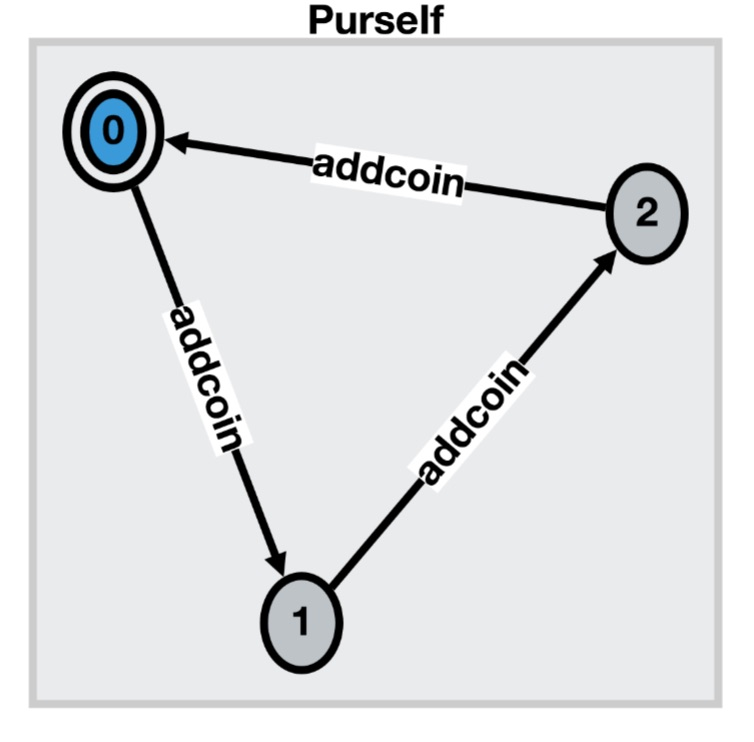
\includegraphics[scale=0.15]{PurseIf.jpg}
\end{minipage}\end{center}

Where as if we use a process that is not event prefixed in a \verb|when| command, see example below, then it fails to parse.
\begin{center}\begin{minipage}{0.5\textwidth}
\begin{verbatim}
PurseW = P[0],
  P[c:0..N] =
   (when (c < N)   addcoin-> P[c+1] |
   when (c >= N)   P[0] ).\end{verbatim}
\end{minipage}\end{center}
}



\subsection{Event indexing}

An indexed event  can be used to model events that input or output values.

A one place buffer that can accept as input a number from the range \verb$1..N$ and then must out put that value is can be represented by an automata with \verb$N+1$ states.

\noindent\begin{center} 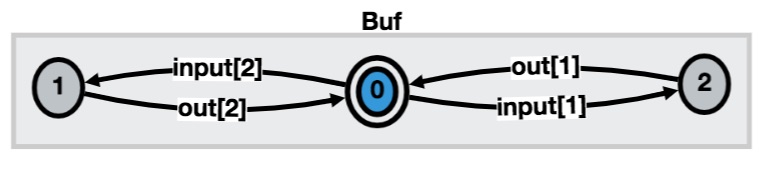
\includegraphics[scale=0.3]{BufI.jpg} \end{center}

The buffer is  defined by:
\begin{center}\verb$Buf = input[v:1..N] -> out[v]->Buf.$\end{center}

The event \verb$input[v:1..N]$  {\bf declares} a new variable \verb|v|  and when it executes  it  {\bf inputs} a value that is assigned to the variable.  The subsequent event \verb|out[v]|  refers to the previously declared variable  \verb|v| and when it is executed it {\bf outputs} the value held in it. So information flows from the \verb|input| event to the \verb|out| event and hence the names.


\subsection{Cars Example}
This example requires  both state and event indexing.
\begin{quotation}
\emph{A car can travel at different speeds and can accelerate at different rates. But no matter how hard it tries to accelerate it can never go beyond its maximum speed.}
\end{quotation}

In this example the car is indexed by its \verb|speed| and  the number on the nodes corresponds to the speed of he car. The rate of acceleration is indexed by \verb|a| and this index  is declared in the event \verb|accelerate|. Hence the rate of acceleration can not appear as an index to the car as that is defined prior to the definition of the event.


\begin{minipage}{0.52\textwidth}
\begin{verbatim}
const N = 3
automata }
Car = C[0],
 C[speed:0..N] =
   (when speed<N  accelerate[a:1..N-1]  ->
        ( if (speed+a<N) then C[speed+a]
           else C[N])
    | when speed>0 brake -> C[speed-1]).
}\end{verbatim}
\end{minipage}
\begin{minipage}{0.35\textwidth}
 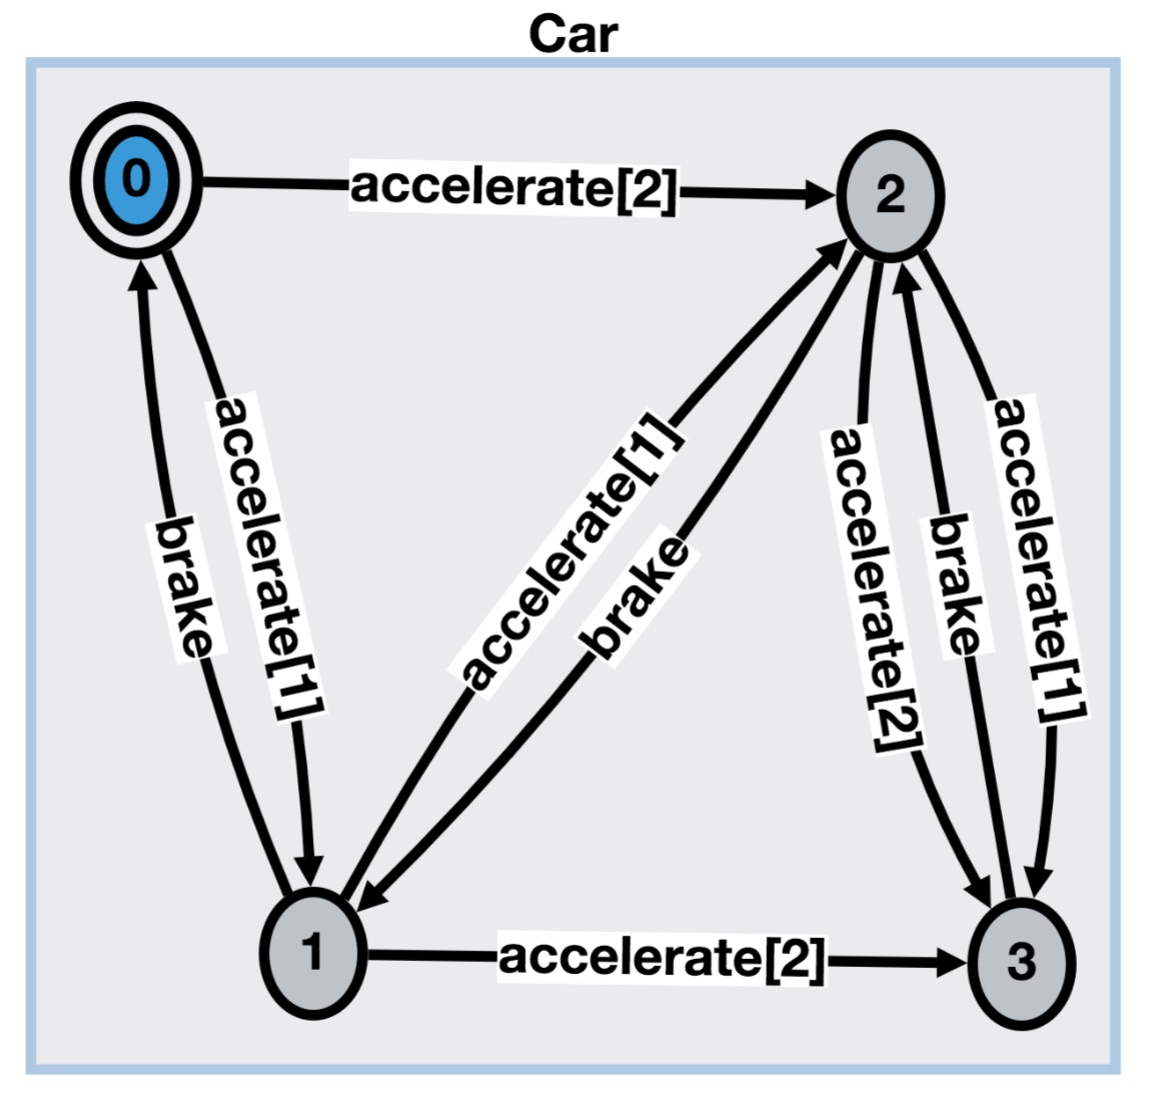
\includegraphics[scale=0.15]{Car.jpg}
 \end{minipage}

In the example above the {\sf Car} has a maximum speed of {\sf 3} and a maximum acceleration od {\sf 2}. But when the {\sf Car} has speed of {\sf 2} the effect of accelerating at {\sf 2} is only to change the speed by {\sf 1}.

 \subsection{From Natural Language to indexed process model}
 Natural languages are expressive but ambiguous.  Added to which we are interested in describing event based models and there is no one universal way to describe such systems. This leads to many problems, some of which can be overcome by breaking the task of formalising these informal specifications into some simple steps.



 {\bf Step 1} find indexes and  indexed states

 {\bf Step 2} find indexed events

 {\bf Step 3} find all events

 {\bf Step 4} build automata
either sketch and code or code and view.

 {\bf Step 5} inspect the automata and validate it against specification

\noindent We will demonstrate this with a simple example of a lockable door.

\begin{quote}
{\it Closed doors are always locked. The door starts closed. The lock can hold any of  a number of  codes.  To open you need to input the correct code and after opening the door can only close. Inputting the wrong code is an error and the door returns its start state. Before using the door the code must be set.

You may assume that only an administrator can set the code  where as any one may use the door by entering codes but such distinctions are not part of the model.
}
\end{quote}

{\bf Step 1} When the numbers of states or events is not fixed but is dependent upon some parameter then you need to build what we call an indexed  process. The parameter is an index and in our example this is the {\sf code} the lock uses. As the code needs to be stored by the Lock we need indexed states \verb|L[j:1..N]|.

{\bf Step 2} There are two indexed events \verb|setlock[k:1..N]| to set the state of the Lock and \verb|enter[ji:1..N]| to enter a code when trying to open the door.

{\bf Step 3} The list of all events: \verb|open,close,error,enter[]| and \verb|setlock[]|

{\bf Step 4} Automata when \verb|N==2|

\noindent\begin{center} 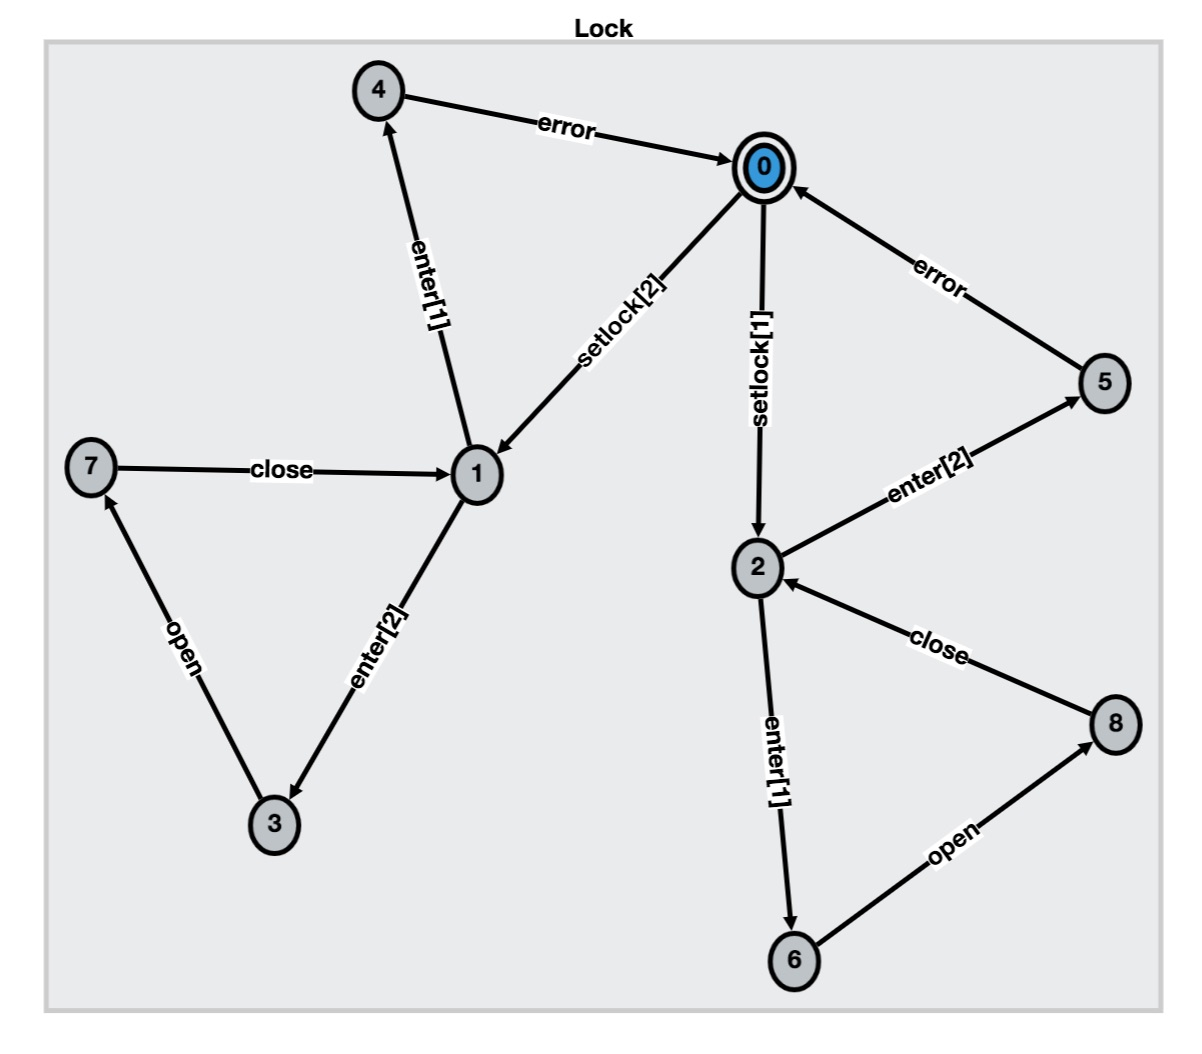
\includegraphics[scale=0.24]{Lock.jpg} \end{center}

This is defined by:

\hspace{1in}\begin{minipage}{0.3\textwidth}
\begin{verbatim}
Lock = (setlock[k:1..N] -> L[k]),
L[j:1..N] = (enter[i:1..N] ->
                   ( when (i==j) open ->close->L[j]
                   | when(i!=j) error->Lock)).   \end{verbatim}
\end{minipage}


{\bf Step 5} Note the value input in the \verb$setlock[i:1..N]$ event is stored in the state of the process \verb$L[i]$ for subsequent comparison with the value input in the \verb$enter[i:1..N]$ event.



  \subsection{Indexing concurrent processes.}
  This means producing an indexed number of concurrent processes but has been implemented in a very restricted. As implemented the indexed process can only communicate with processes that are running in parallel with them. Alas they cannot communicate with each other.


  If you want \verb$N Worker$ processes, each  labeled with \verb$[1],[2],...[N]$

 \begin{center}\begin{minipage}{0.55\textwidth}
\begin{verbatim}
Worker = (getTask -> doTask -> Worker).
Workers = (forall [i:1..N] ([i]:Worker)).
   \end{verbatim}
\end{minipage}\begin{minipage}{0.4\textwidth}
\begin{center}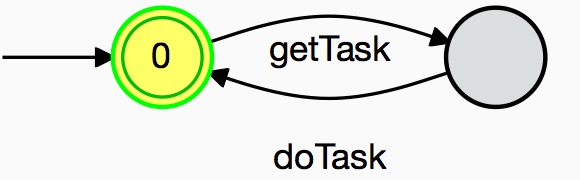
\includegraphics[scale=0.3]{Worker.jpg}\end{center}
\end{minipage}

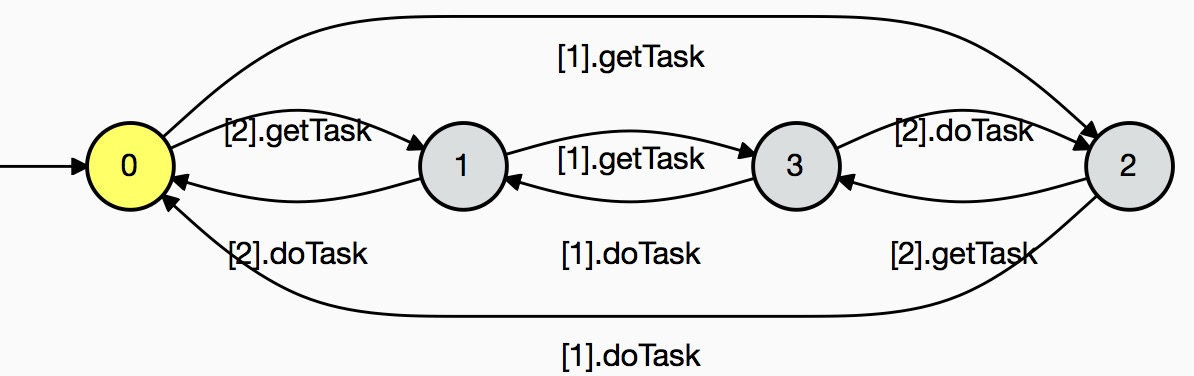
\includegraphics[scale=0.3]{Workers.jpg}
\end{center}

 We can add a \verb$Farmer$ process to hand out the \verb$Task$s to the \verb$Worker$s in order. Then  build a \verb$Farm$ composed of the \verb$Farmer$ and the \verb$Workers$.

\begin{center}\begin{minipage}{0.55\textwidth}
\begin{verbatim}
 Farmer = F[1],
  F[i:1..N] = (when (i<N) [i].getTask->F[i+1]
             | when (i>=N) [i].getTask->F[1]).

Farm = (Farmer || Workers).
   \end{verbatim}
\end{minipage}\begin{minipage}{0.4\textwidth}
\begin{center}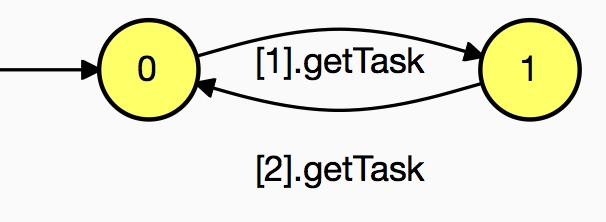
\includegraphics[scale=0.275]{Farmer.jpg}\end{center}
\end{minipage}
\end{center}

The \verb$Farmer$  process is far from ideal in some regards.

\section{Petri Nets  {\color{red} 2b added 2017}}
{\color{red}


What we refer to as a Petri Net is actually an extension of Petri Nets with labels on the  transition.  This appear in the literature under the name of the \emph{Box calculus}. Our definition of parallel composition is not a part of main stream Petri Nets but a part of the Box calculus.

{\color{blue}
\emph{{\bf A Petri Net} is a tuple  $\sf A \triangleq (P_A,S_A,T_A,Arcs_A,\alpha_A,Name_A)$  where:
\begin{description}
\item[$\sf P_A$] is the set of places,
\item[$\sf S_A$] is the set of  initial  Markings $\sf M_A\subseteq S_A$ where a Marking is  a set of placess $\sf M_A\subseteq P_A$
\item[$\sf T_A$] is the set of transitions
\item[$\sf Edges_A$] Edges join node to transitions and transitions to nodes. There can be multiple places joined to a single transition and multiple transition joined to a single place.
\newline
$\sf Edges_A\subseteq \{(p,t): p\in P_A, t\in T_A \}  \cup \{(t,p): p\in P_A, t\in T_A \}$
\item[$\sf \alpha_A$] is the alphabet of the process
\item[$Name_A$] a transition naming function $\sf Name_A:T_A\rightarrow \alpha_A$
\end{description}
}
$\Box$
}


 \subsection{Appearance}
 Nets have  Places, large circles,  not nodes and the initial state of a Petri Net is a set of places each  \emph{marked} with a  token, a small black circle. The transitions are represented by Boxes and event names. Arcs are added from \emph{pre place}, ${\sf\bullet t}$ to the Box of transition {\sf t}  and from transition {\sf t} Box  to \emph{post place} ${\sf t\bullet}$.

Finite state Petri Nets  like finite state automata can be  approximation of potential infinite sate processes. The location of the Petri net transitions is the same as that for Automata.

There is a simple relation between finite state sequential automata and finite state Petri Nets. In addition the definition of event hiding and event renaming   on Petri Nets and its relation to event hiding and event renaming   on  automata is quite obvious.



Our tool takes process specifications $\mathcal{P}$ and builds finite state automata {\sf P}. But now we want to build Petri Nets from specification ${\sf Petri(\mathcal{P})}$. The operations defined on atomic processes can be lifted to operations on Petri Nets.

Parallel merge of two processes, parallel composition with no synchronisation is just the union of the component nets. Hence automata node is represented by a marking. That is a pair of places, one element of the pair taken from each component process. Thus each place represents the state of one of the component processes. Each process can be give a unique location and then each node annotated with the location of its process.
The start node corresponds to the the pair of initially marked places.

Event synchronisation of $t_1$, $\aro{\bullet t_1}{a}{t_1\bullet}$ and $t_2$, $\aro{\bullet t_2}{a}{t_2\bullet}$ is a new transition $t_3$ with the same name and with pre places the union of the component transitions pre places. The post places are constructed similarly.
\[t_3\triangleq \aro{(\bullet t_1\cup \bullet t_2)}{a}{(t_1\bullet \cup t_2\bullet) }\]




\subsection{Token Rule}


 We define \verb|TokenRule| that maps Petri Nets to atomic processes and must preserve the transition  locations.  These are the same automata that would have been constructed had we built the automata directly from our process language, hence we have:

\[{\sf TokenRule(Petri(\mathcal{A}))\sim  \mathcal{A}}\]

Let us write {\sf A} and {\sf B} for Petri Nets. We have   lifted   operations ${\sf Op_a}$ on automata to   operations ${\sf Op_n}$ on Petri Nets  so that they obey  the following algebraic rules:

\[{\sf TokenRule({\sf A}\parallel_n {\sf B})\sim  (TokenRule({\sf A})\parallel TokenRule({\sf B})) }\]

\[{\sf TokenRule({\sf A}\$\{x\}) \sim  (TokenRule({\sf A}))\$\{x\}  \qquad     TokenRule(abs({\sf A}))\sim  abs_n(TokenRule({\sf A})) }\]


The \verb|TokenRule|  builds an automata from a Petri Net by executing transitions of the Petri Net.  A Petri Net transition can only  be executed when all its pre places are marked. When the transition is executed the tokens on its pre places are removed and tokens are placed on the transitions post places.

Above explains how an atomic specification can be used to build a Finite State Petri Net, FSPN.  The construction of FSPN from indexed specifications  proceeds by constructing the FSPN for each sequential process analogously to the construction of finite state automata.

We can compute, {\sf PTokenRule},  a \emph{partial Token Rule} that takes a set of process names that must be converted into an automaton  prior to applying $\_\parallel_n\_$ to build a Petri Net from the newly built sequential Net and the remaining Petri Nets.


\subsection{From Automata to Petri Nets}
Building Petri Nets from automata with located transitions {\sf LA2PN} works as follows:

{\bf Suggestion 1 *The direct assault is Not So Good*}
Note the Interleaving Merge of {\bf N processes} builds  an Automata that is an {\bf N-dimensional} cube. The first thing you need to do is identify the start and end "corners".

\vspace{1em} \begin{minipage}{0.2\textwidth}
\begin{verbatim}
A=a->(b->STOP|
          c->STOP).
B=aa->(bb->STOP|
          cc->STOP).
S= A||B.
  \end{verbatim}
\end{minipage}
\begin{minipage}{0.6\textwidth}
\begin{center}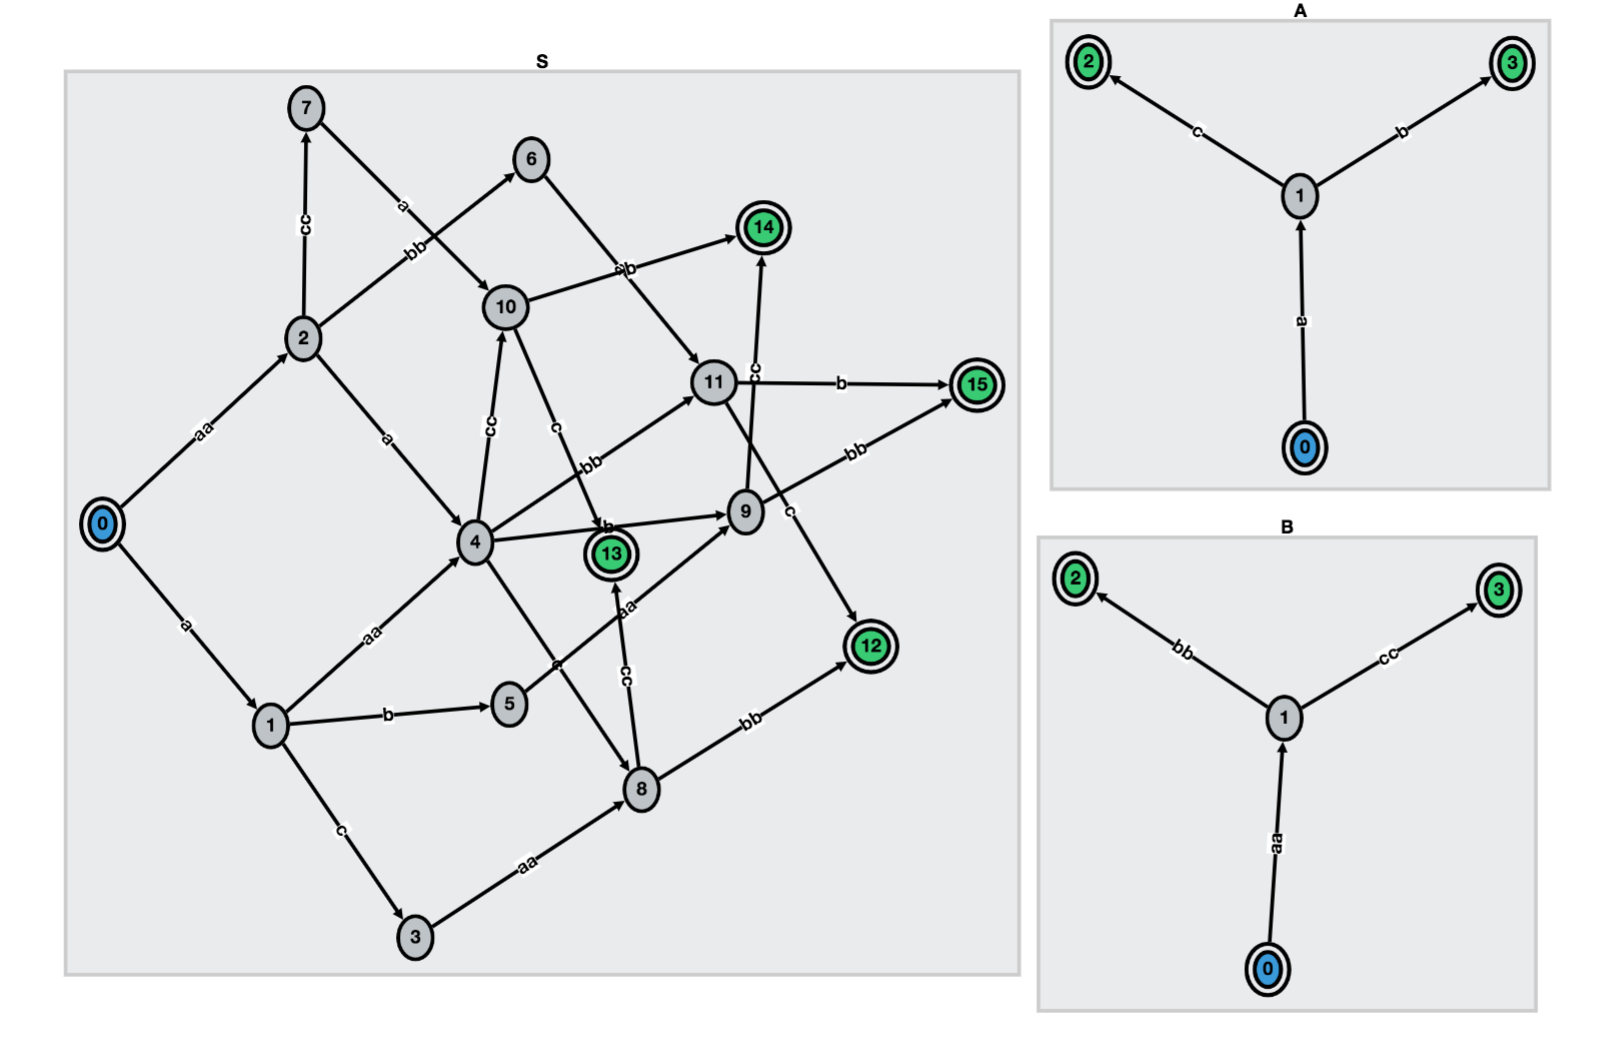
\includegraphics[scale=0.4]{Surface.png}\end{center}
\end{minipage}

In the above example the start and end corners are marked with blue and green nodes. But this is because the "cubes" are the whole automata. What is required is to find these cubes.

 Let {\sf Loc(A) = 1, Loc(B)=2} in above.   Add the root {\sf 0} to the TODO list. For each element in TODO list compute the surfaces if  we have  two transitions with disjoint location leaving  so compute $\sf \{0,1,2,4\}$. Remove $\sf 0$ from the TODO list and add nodes ${\sf \{1,2,4\}}$ to the TODO list.  When
$\arop{n}{\_}{x}{l}$,  $\arop{m}{\_}{x}{k}$, ${\sf  l \notin Loc(Next(n))}$ and ${\sf  k \notin Loc(Next(m))}$ then {\sf x} is ${\sf \{1,2\}}$ end!

Question with {\sf n} distinct locations, $\sf \{1,2,3,4,\ldots n\}$ ?
\begin{enumerate}
\item split into location {\sf 1} and locations $\sf \{2,3,4,\ldots n\}$ and build two Petri nets then split the Petri Net for locations $\sf \{2,3,4,\ldots n\}$.
\end{enumerate}
Having done this the cubes can be converted into Petri Nets and joined together.

{\bf Suggestion 2 *Looks Good*} Step 1 approximation build separate Nets one for each location, splitting the  synchronised events into components. Where {\bf twists} occur make cross product of places.

Note we glue automata together by glueing two nodes together and with Petri Nets we need to glue to markings together. This is done by building the cross product of  two sets of tokens.

{\bf Suggestion 3}   Define a Location space where each location is a subset of primitive locations. Build a Place for each primitive location an start adding transitions by adding pre arcs for each primitive. Th e post arcs are added to new Places of each primitive  location. When the automata returns to an existing state  glue the corresponding Markings together.

Simplify the Net  by pruning merging identical Places then by pruning identical Transitions.  Review!

{\bf Some  tests:}
\[{\sf A\sim  TokenRule(LA2PN(A))}\]

\subsection{Indexed Petri Nets}

Indexed, specifications can be turned into FSPN in two quite separate ways. For a sequential indexed process $\mathcal{P_I}$ :
\begin{enumerate}
\item expand the  index $\mathcal{I}$ converting $\mathcal{P_I}$ into  a sequential FSPN
\item turn the index $\mathcal{I}$ into a FSPN and the sequential process $\mathcal{P}$  into another  then build, $\mathcal{P}\parallel_n \mathcal{I}$,  net parallel composition of  the process and the index.
\end{enumerate}
Both options and be applied to  {\sf PTokenRule} the partial expansion of a net into an automata.
All options  should result in interleaving equivalent Petri Nets.

Can we define Petri Net bisimulation so that:

\[{\sf Petri(\mathcal{A}\parallel \mathcal{B} ) \sim_n  (Petri(\mathcal{A}))\parallel_n Petri(\mathcal{B}))   }\]

\[{\sf Petri(\mathcal{A}\$\{x\}) \sim_n  (Petri(\mathcal{A}))\$\{x\}  \qquad     Petri(abs(\mathcal{A}))\sim_n  abs_n(Petri(\mathcal{A})) }\]


\subsection{Hiding and simplifying  Nets}
Tow options
\begin{enumerate}
\item define abstraction and bisimulation on nets OR
\item use {\sf LA2P} the mapping from located automata to Petri Nets.
\end{enumerate}
An advantage of using located Automata and Nets is that event refinement can be defined.

}
\section{ Symbolic Processes  {\color{red} mostly 2b added 2017}}
Simple process specifications, those with out indexes, are "atomic" specifications that produce atomic automata.   An atomic  automata has atomic transitions with  a single atomic name and  a finite set of  atomic  nodes each   representing  one state.

Indexed process specifications represent processes with variables, the indexes, and may be infinite state. The indexed specifications are expanded to a finite state approximation of the underlying and potentially infinite state automata. They do this using defined bounds such as \verb|const N = 4|.


Alternatively we could define symbolic automata, automata with variables.
The state of  the process, represented by a symbolic automata, is   the pair $(n,\mu)$ where $\mu$ is an  evaluation i.e. a mapping from variables to values and n is a node of the automata.

\[\mu: Var \rightarrow Val\]
Hence the node of a symbolic transition only tells you part of the state of the process. When a event of a symbolic process is actually executed the state of the process both moves from the pre-node of the transition to the post-node of the transition and the evaluation of the variable changes as defined by the assignment.  Symbolic execution represents a whole set of actual executions.

The symbolic  transitions need  to be annotated  with its name plus a boolean guard and an assignment. Let a transition  ${\sf t1 \triangleq (n1,g1,ev1,a1,m1)}$  be represented as
\[{\sf n1\xrightarrow{\text{\sf g1,ev1,a1}} m1}.\]
Both the guards {\sf g1} and assignments {\sf a1} may contain the process variables.  Note symbolic Petri Nets can be built by adding the variables from a process to the places that represent the state of that process.

Our tool takes process specifications $\mathcal{P}$ and,  by default, builds finite state automata {\sf P}. But now we want to prevent the expansion of indexes and build symbolic automata  from the specification ${\sf \mathcal{P}\$\{x\}}$.

The execution of a guarded  event  can only occur when the guard is true  and then the assignments of the transition are applied hence building another evaluation. Two  essential functions needed in the definition of the application of assignments {\sf a}, writen  $\_@{\sf a}$ are:
\begin{enumerate}
\item syntactic substitution and
\item simplification.
\end{enumerate}

Simplification certainly needs to be out soured to proof services as  many decades of work has gone into developing such algorithms. And doing this allows for the development of theories of specific data types that include both their definition and the proof of rules of inference used in simplification. Essential this provides an extensible proof engine.

Syntactic substitution look easy but  either you need to; hard bake in the language the data types used or out source both  parsing and substitution. \emph{Initially hard bake in integers, lists and sets?}

Reasoning about symbolic processes requires that we can concatenate sequential transitions. This can be achieved using  two basic standard techniques, \emph{symbolic execution} and backward reasoning via \emph{Hoare Logic}. Hoare Logic tells us how to compute the weakest precondition prior to an assignment ${\sf ass}$ of  a post condition ${\sf bg}$ and is written  ${\sf bg@ass}$.  Whereas symbolic execution tell us how to combine the sequential execution of two assignments ${\sf a1}$ and then ${\sf a2}$ into a single assignment that is written ${\sf a1@a_2}$

Let assignment ${\sf ass}$ be a set of assignments all applied in parallel $\{x:=E,y:=F\}$ and let semicolon be used to compose assignments sequentially.

Compute the weakest precondition of an assignment for a known post condition:
\[ \{P[E/x]\} x:=E \{P\} \]
In our notation the precondition  $P@\{x:=E\}\triangleq P[E/x]$

Use symbolic execution to remove the sequencing of assignments.

\[ x:=F(x,y); y:=G(x,y)  = \{x:=F(x,y), y:=G(F(x,y),y)\}\]

In our notation $  \{x:=F(x,y)\}@\{y:=G(x,y)\}  \triangleq  \{x:=F(x,y), y:=G(F(x,y),y)\}$


\section{ Index freezing   (z3  -  headless Isabelle)}

{\bf Closely related to Petri net Construction and Token Rule.}

The default interpretation, semantics, of an indexed process definition is its finite state expansion using the declared values of the parameters. An alternative interpretation is to not expand some indexes but to leave them as unknown and define symbolic events.


\begin{minipage}{0.55\textwidth}
\begin{verbatim}
S1 = X[0],
  X[x:0..N]=(when (x<N) out[x]->X[x+1]|
              when (x==N) stop->STOP).
S = S1${x}.
   \end{verbatim}
 \vspace{-2em}{\color{red}
 \begin{enumerate}
 \item assignment \verb|x:=x+1| is missing
 \item presentation order \emph{guard name assignment}
 \item \verb|2| should be \verb|N| and \verb|$x| should be \verb|x|
 \end{enumerate} }
\end{minipage}\begin{minipage}{0.4\textwidth}
\begin{center}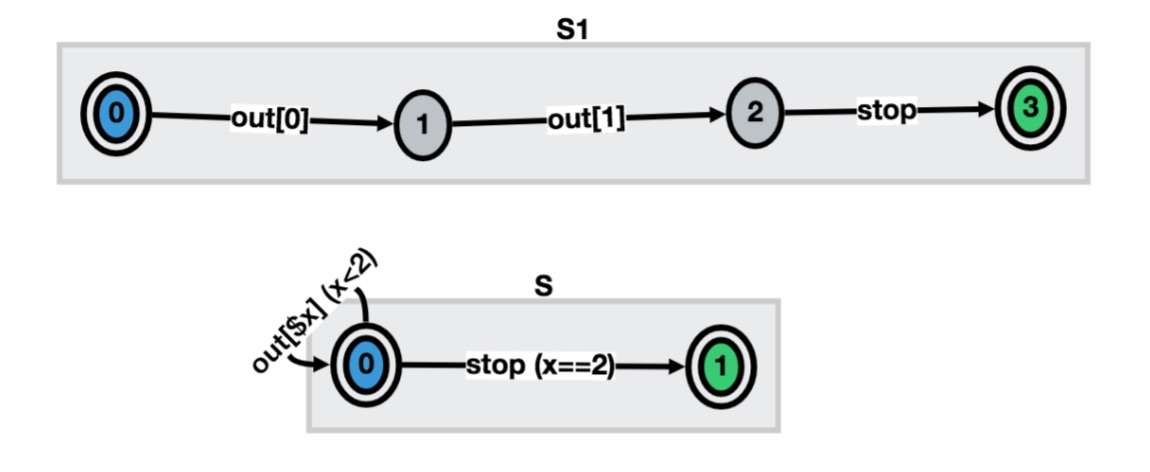
\includegraphics[scale=0.2]{VarBug.jpg}\end{center}
\end{minipage}



For the parallel composition of indexed processes we will need to $\alpha$ convert index names to prevent name clashes. This can be achieved by profixing an index name with its process name, hence \verb|x| above would become \verb|S1.x|

\vspace{1em} \begin{minipage}{0.55\textwidth}
\begin{verbatim}
R1 = input[y:0..N] -> X[y],
  X[x:0..N] = (when (x<N) out[x] -> X[x+1]|
              when (x==N) stop ->STOP).
R = R1${x}.
T = R1${x,y}.
S = R1${y}.
   \end{verbatim}

 \vspace{-3em}{\color{red}\begin{enumerate}
   \item \verb|S = R1${y}|  currently fails to build.
   \end{enumerate}
   }
\end{minipage}
\begin{minipage}{0.4\textwidth}
\begin{center}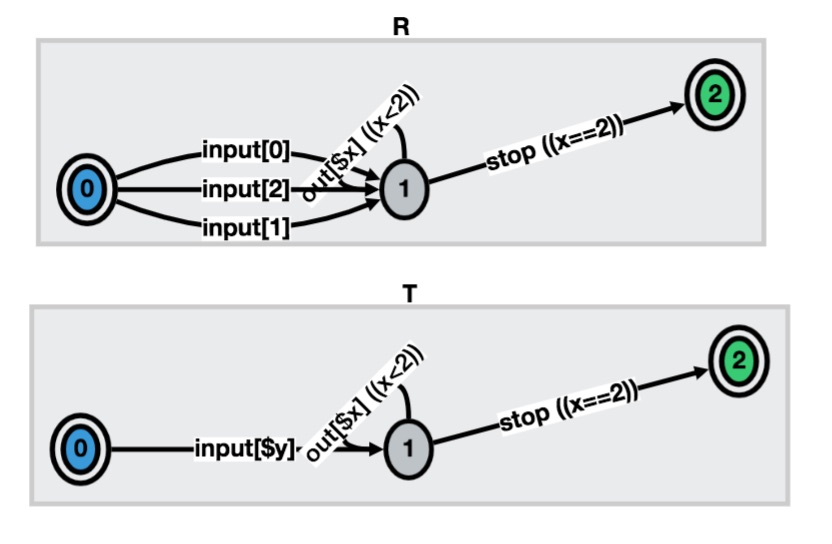
\includegraphics[scale=0.2]{VarBug2.jpg}\end{center}
\end{minipage}

In the above example both indexes {\sf x} and {\sf y} are needed.

\vspace{1em} \begin{minipage}{0.55\textwidth}
\begin{verbatim}
Lift = L[0][0],
  L[x:0..N][to:0..N] = btnto[i:0..N] -> L[x][i]  |
       when (x!=to) move ->L[to][to].
  \end{verbatim}

All three Indexes {\sf x}, {\sf to} and {\sf i}  are needed.
\end{minipage}
\begin{minipage}{0.4\textwidth}
\begin{center}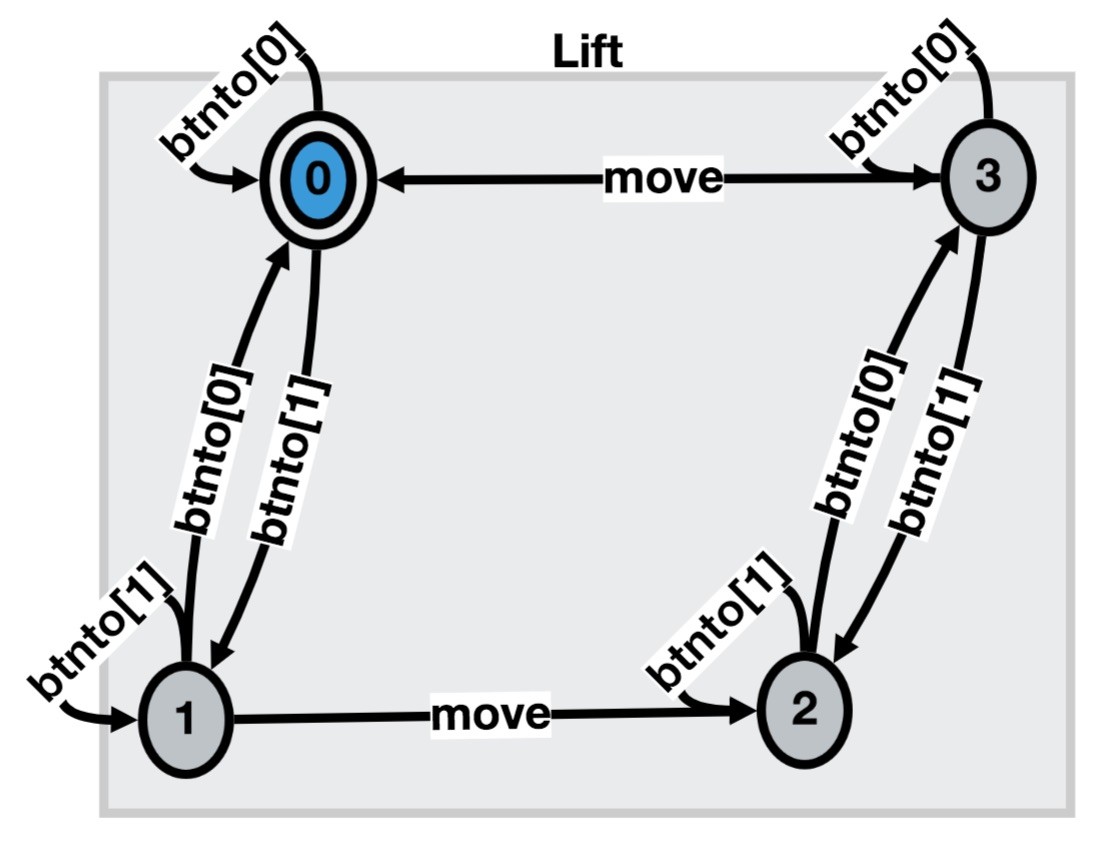
\includegraphics[scale=0.12]{Lix.jpg}\end{center}
\end{minipage}



Need a symbolic expansion mapping,  \verb|S2A|  that takes as input a symbolic  automata and returns an atomic automata.




\begin{center}
\begin{minipage}{0.3\textwidth}
\begin{verbatim}
R = R1${x}.
T = S2A(R{x}).
\end{verbatim}
\end{minipage}
\end{center}

The result of expanding all variables should be the same as building the atomic automata from  scratch, hence \verb|R|$\sim$\verb|T| in above. (Note building from the automata/Petri Net allows interacting with the diagram)




\subsection{Need for index freezing }
{\color{red}

\begin{minipage}{0.55\textwidth}
{\bf Take a look at the examples} below.

\begin{verbatim}
const N = 1
automata {
Buf1data = input[i:1..N] -> F[i],
   F[d:1..N] = output[d] -> Buf1data.
Buf2a = (a:Buf1data)/{b.move[x:1..N]/a.output[x]}.
Buf2b = (b:Buf1data)/{b.move[x:1..N]/b.input[x]}.

B2indexed = Buf2a||Buf2b.
Bu2x = B2indexed${x}.
}
   \end{verbatim}
\end{minipage}\begin{minipage}{0.35\textwidth}
\begin{center}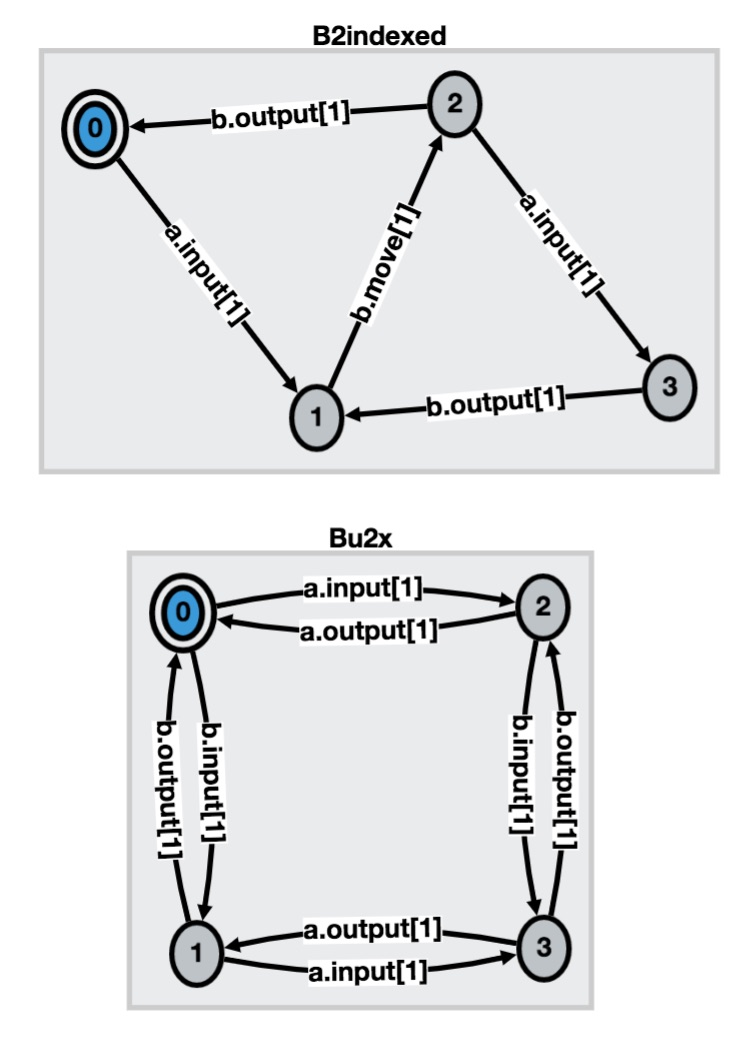
\includegraphics[scale=0.17]{hideB.jpg}\end{center}
\end{minipage}

The two place buffer that, in each place can only hold the number 1.

What I do not understand is how \verb|B2indexed| dose not have event  \verb|a.output[1]| but
\verb|Bu2x = B2indexed${x}.| dose?



{\bf A more complex example} is:

\begin{minipage}{0.55\textwidth}
\begin{verbatim}
const N = 3
automata {
Buf1data = input[i:1..N] -> F[i],
   F[d:1..N] = output[d] -> Buf1data.

Buf2a = (a:Buf1data)/{b.move[x:1..N]/a.output[x]}.
Buf2b = (b:Buf1data)/{b.move[x:1..N]/b.input[x]}.

Buf2data* = Buf2a||Buf2b.
Buf2 = simp(abs(Buf2data\{b.move[x:1..N]})).
//B2 = Buf2${x}.
B2indexed = (Buf2a||Buf2b)\{b.move[q:1..N]}.
Temp = B2indexed /{input/a.input[x:1..N],
                   output/b.output[x:1..N]}.
BestGuess = simp(abs(Temp)).
//Bu2x = B2indexed${x}.
}
operation {  Bu2x ~ BestGuess.}
   \end{verbatim}
\end{minipage}\begin{minipage}{0.4\textwidth}
\begin{center}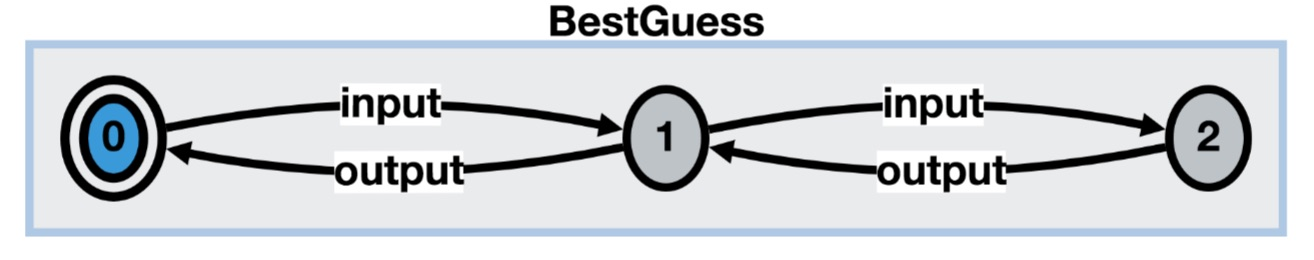
\includegraphics[scale=0.15]{BestGuess.jpg}

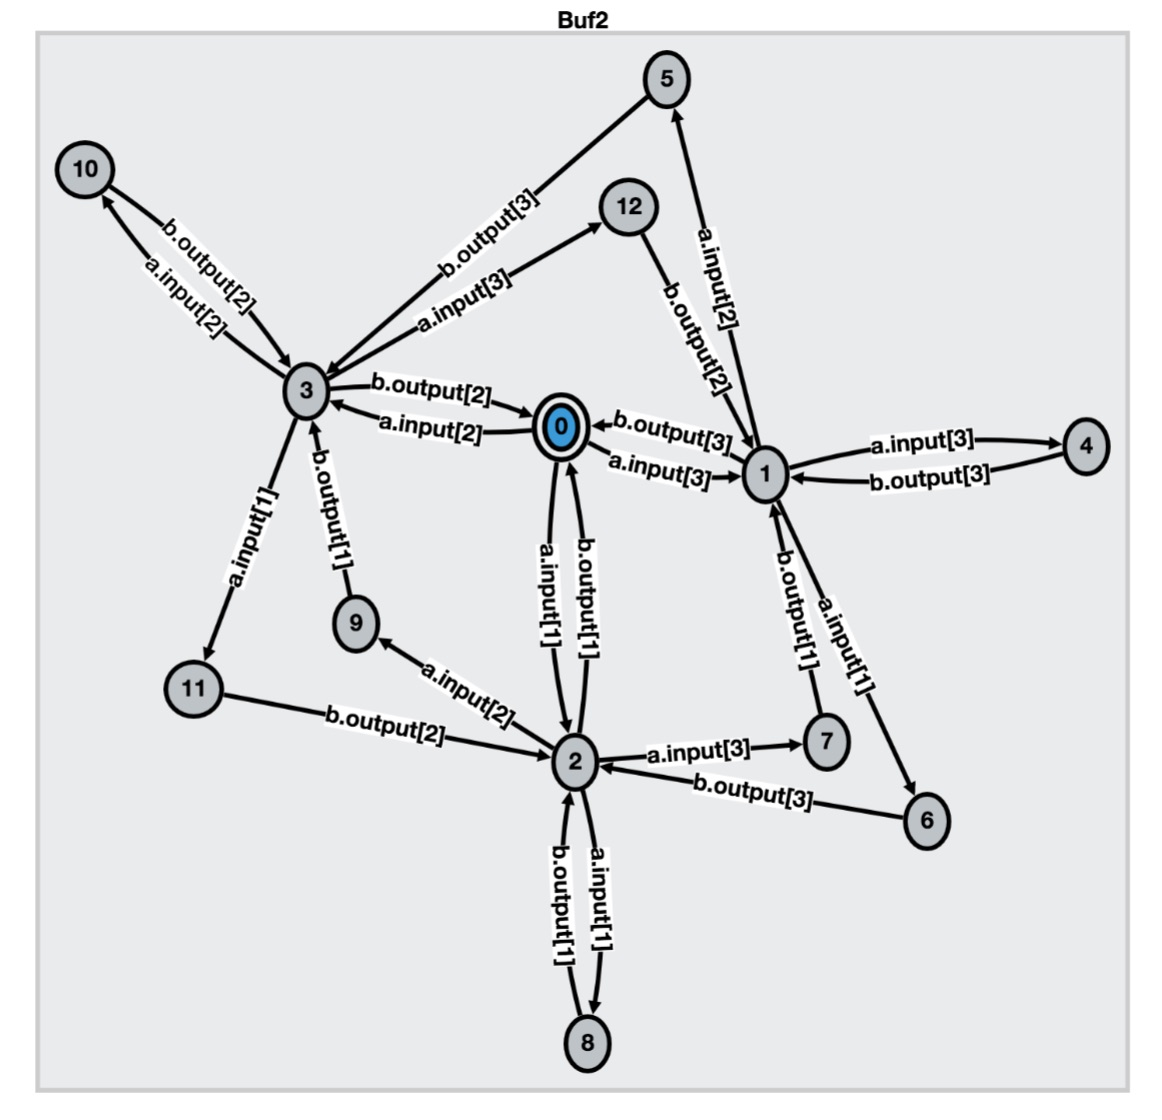
\includegraphics[scale=0.17]{HideBuf2.jpg}\end{center}
\end{minipage}

The two place buffer that, in each place can hold a number from $\{1,2,3\}$ is defined and displayed.  It is not as easy to see that it is a buffer as I wild like and if we could \emph{freeze} the data in each place we might have simpler visual representation.


This will require some work to achieve.  One tracking  indexes so that we know what indexes exist in a process. For example what indexes are in \verb|Buf2| defined above? Hence what should we write

\verb|B2 = Buf2${x}|
}



\subsection{Symbolic 2 Atomic mapping S2A}
Symbolic execution  is the obvious way  to  map \verb|S2A|  Symbolic Processes  to  Atomic Processes.

\[{\sf S2A(A\$\{x\})\sim  A }\]

State contains  an evaluation of the variables.


All you need to do is build a new node for each distinct evaluation reached.

 \begin{quote}
 Add  the set of initial evaluations to a "to do list" and repeatedly:

 \emph{Remove the top node from the to do list and evaluate the boolean guard of each  symbolic event and those that evaluate to true you apply the assignment to compute the new reachable state. If the new state already exists then add the transition ending at the corresponding  node else add the state.  When  all events of the selected node have been processed either select the next node on the to do list else if the list is empty terminate.  }
 \end{quote}




Reasoning about symbolic systems is problematic as they are infinite state and consequently frequently require a degree of theorem proving. A vast amount of work has gone into both push button theorem proving and interactive theorem proving over the recent years.  Yet push button theorem needs to be a lot stronger and interactive theorem proving a lot easier.

{\bf To code with data structures, such as lists and records,  needs headless Isabelle.}  Initially we will only have Z3 and are restricted to integers.  For data structures  we need rules for rewriting, simplifying, the data structures. These rules constitute a \emph{Theory} of the data structure and as they are heavily reused are defined and stored on file. Thus a procedure should import them  not define them.




\subsection{Symbolic parallel composition $\_\parallel_s\_$}
The operations defined on atomic processes can be lifted to operations on symbolic processes. We first define \verb|S2A| that maps symbolic process to atomic processes and then lift  the atomic  operation ${\sf Op_a}$ to the symbolic operation ${\sf Op_s}$ so that:

\[{\sf S2A(Op_s(A,B))\sim  Op_a(S2A(A),S2A(B)) }\]

Symbolic parallel composition $\_\parallel_s\_$ is an extension of  atomic parallel composition $\_\parallel\_$ where:
\begin{enumerate}
\item the nodes have a union of the indexes, suitably renamed to prevent name clashing
\item synchronising transitions have guards the conjunction of the component guards and assignments the union of the component assignments.
\end{enumerate}


\subsection{Symbolic abstraction}


Let a transition  ${\sf t1 \triangleq (n1,g1,ev1,a1,m1)}$  be represented as   ${\sf n1\xrightarrow{\text{\sf g1,ev1,a1}} m1}$. We may refer to {\sf n1}  as ${\sf t1_{pre}}$,  to {\sf m1}  as ${\sf t1_{post}}$ and refer to {\sf e1}  as ${\sf t1_{en}}$.

We need to  compute $\sf t1: t2$  the transition representing the execution of $\sf t1$ followed by $\sf t2$.  The execution of two transitions one after the other only occurs if the port node of the first transition is the pre-node of the second transition.

%$ \AroL{1}{2222222}{3}{4} $

% $\AroL{\sf n}{\text{g1,ev1,a1}}{m}{x} $

% ${\sf m\yrightarrow{\text{b2,ev2,a2 }} o}$

\begin{center}\begin{minipage}{0.75\textwidth}
\inference[$t_1: \tau$:]
{
{\sf n\xrightarrow{\text{\sf g1,ev1,a1}} m} \quad  {\sf m\xrightarrow{\text{\sf g2,$\tau$ ,a2 }} p}
}
{{\sf n\xRightarrow{\text{$\sf g1\land g_2@a_1,ev1,a1@a_2$}}p }}
\end{minipage}
\qquad
\begin{minipage}{0.75\textwidth}
\inference[$\tau: t_2$:]
{
{\sf n\xrightarrow{\text{\sf g1,$\tau$,a1}} m} \quad  {\sf m\xrightarrow{\text{\sf g2,ev2 ,a2 }} p}
}
{{\sf n\xRightarrow{\text{$ \sf g1\land g_2@a_1,ev2,a1@a_2$}}p }}
\end{minipage}\end{center}


The guard ${\sf g2}$ is the post condition to transition ${\sf t_1}$ hence to compute the weakest precondition we need to apply Hoare Logic thus compute ${\sf g_2@a_1}$  which we add as a conjunction to the guard of ${\sf t1}$.  Thus  if ${\sf t1_{pre} = t2_{post}}$   we can add the transition :
\[t1: t2 = \sf (t1_{pre}, t1_g\land t2_g@t1_a , t1_{en}:t2_{en}, t2_a@t1_a, t2_{post})\]
but if  ${\sf t1_g\land t2_g@t1_a\neq False}$ then this transition can never be executed and hence can be removed with out effecting the behaviour of the process.

We can construct tests from:
\[{\sf S2A(abs(P))\sim abs(S2A(P))}\]



\subsection{Symbolic simplification}
We certainly want property:
\[{\sf S2A(simp(P))\sim simp(S2A(P))}\]
this could certainly be achieved if symbolic bisimulation simply matched transitions $t1$ and $t2$ by
\[t1_b\Leftrightarrow t2_b \land t1_{en}= t2_{en} \land t1_a\Leftrightarrow t2_a.\]
It might be possible to further simplify the symbolic automata while preserving the stated property.


\section{Symbolic Petri Nets {\color{red} 2b added 2017}}

The symbolic Petri Nets  are an \emph{orthogonal} combination of the symbolic extension to automata and the construction of Petri Nets rather than automata. Thus we have a square with finite automata, finite Petri Nets, symbolic automata and symbolic Petri Nets on the corners. Mappings between adjacent edges  are functions that should preserve the semantics of the processes, be monotonic with respect to refinement and congruent with respect to the operators.



\begin{center}
\begin{minipage}{0.4\textwidth}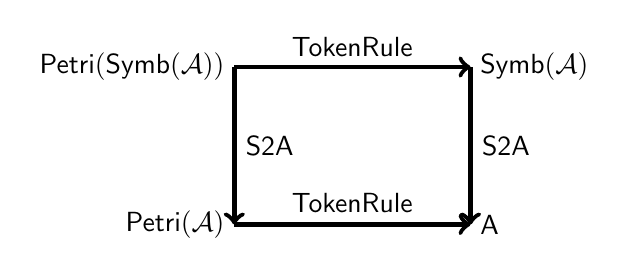
\begin{tikzpicture}
\coordinate [label=right:{\sf A}] (A) at (3,0);
\coordinate [label=left:{$\sf Petri(\mathcal{A})$}] (B) at (0,0);
\coordinate [label=right:{$\sf Symb(\mathcal{A})$}] (C) at (3,2);
\coordinate [label=left:{$\sf Petri(Symb(\mathcal{A}))$}] (D) at (0,2);
\draw [line width=0.6mm,<-](A) -- (B) node [midway,above,sloped] {\sf TokenRule};
\draw [line width=0.6mm,<-](C) -- (D) node [very thick,midway,above,sloped] {\sf TokenRule};
\draw [line width=0.6mm,<-](A) -- (C) node [midway,right] {\sf S2A};
\draw [line width=0.6mm,<-](B) -- (D) node [midway,right] {\sf S2A};

\end{tikzpicture}\end{minipage}
\begin{minipage}{0.4\textwidth}
\[{\sf S2A(Petri(\mathcal{A}\$\{x\}))\sim  Petri(\mathcal{A}) }\]
\[{\sf TokenRule(Petri(\mathcal{A}\$\{x\}))\sim  \mathcal{A}\$\{x\}}\]
\end{minipage}
\end{center}

Index freezing prevents the building of  finite state approximations of the index and instead builds a symbolic process. The construction ${\sf Symb(\_)}$ freezes all indexes but in the above square could be replaces by the more general index freezing ${\sf  \_\$\{x,..\}}$ of any set of indexes.

We have seen the partial expansion of both Petri Nets and of symbolic automata an clearly this can be generalised to a partial expansion of Symbolic Petri Nets.

\newpage
{\color{red}
\section{Statefull syntax}
\begin{enumerate}
\item Declare constants in each process
\item Declare variables in each process
\item Process = process name, indexed process or {\bf assignment statements}
\item {\bf guard event $->$ process} OR  {\bf event = guard  process}
\end{enumerate}

\subsection{Translation:}

\begin{center}  \begin{minipage}{0.5\textwidth}
\begin{verbatim}CM = (teaButton->takeTea->STOP
       |coffeeButton->takeCoffee->STOP).\end{verbatim}
\end{minipage}
\begin{minipage}{0.45\textwidth}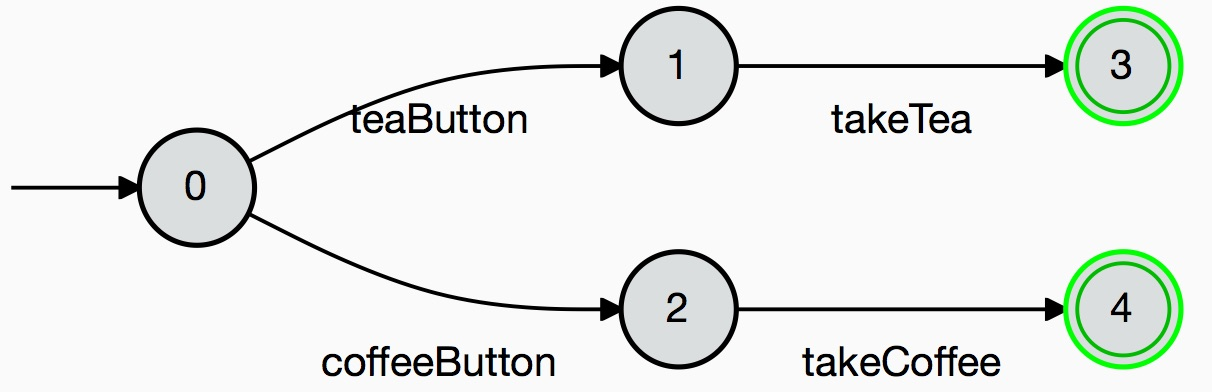
\includegraphics[scale=0.15]{CM.jpg}
\end{minipage}\end{center}

Introduce a variable \verb|St| to distinguish different processes (nodes).

\noindent\begin{minipage}{0.5\textwidth}
 \begin{verbatim}
 CM = const N;
     var St:0..N;
     init = St:=0;
     events =
       when(St==0) teaButton->St:= 1
      |when(St==0) coffeeButton->St:= 2
      |when(St==1) takeTea->St:=3
      |when(St==2) takeCoffee->St:= 4.
 \end{verbatim}
 \end{minipage}
 \begin{minipage}{0.45\textwidth}
 \begin{verbatim}
 CM = const N;
    var cnt:0..N;
    init = cnt:=1;
     teaButton = when(St==0) St:=1
     coffeeButton = when(St == 0)  St:=2
     takeTea = when(St == 1)  St:=3
     takeCoffee =when(St == 2)  St:=4.
   \end{verbatim}

 \end{minipage}




\begin{enumerate}
\item \verb|C[1]| into initialise first index to \verb|1|
\item  \verb|C[cnt:1..N] = ...|  into declaration of \verb|cnt| at first index and rhs as process definition
\item \verb|C[cnt+1]| into  process after \verb|cnt:=cnt+1|.
\end{enumerate}

\begin{center}\begin{minipage}{0.45\textwidth}
\begin{verbatim}
Money = const N;
    var cnt:0..N;
    init = cnt:=1;
    events =
      when(cnt<N) coin -> cnt:=cnt+1
     |when(cnt==N) coin -> cnt:=1.
\end{verbatim}
\end{minipage}
\begin{minipage}{0.45\textwidth}
\begin{verbatim}
Money = const N;
   var cnt:0..N;
   init = cnt:=1;
   coin = when(cnt<N) cnt:=cnt+1
         |when(cnt==N) cnt:=1.
  \end{verbatim}
\end{minipage} \end{center}
}
\newpage
\section{Semantic equivalence  of processes}
One of the key questions is:  what automata should be equated and how do you justify you notion of equality? Before we try to answer this we need to remember what equality means.

 \subsection{Classic notions of equality}   A equality is a relation between  items from some domain, here we are interested in process equality so the domain is the set of all processes. Equality has the following properties:
 \begin{enumerate}
 \item an equivalence relation, a reflexive, symmetric and transitive relation
 \item substitutive and
 \item where equivalent objects are indistinguishable.
 \end{enumerate}

Indistinguishable processes  can be formalised as \emph{testing equivalent}. Substitutive can be formalised are congruent w.r.t. process operators, from a practical perspective the most important being parallel composition.


 \subsection{Complete Trace equality}
 See \sref{Trc} for details.

 This can be computed by the well documented \emph{Subset Construction} that computes a Deterministic automata from a non deterministic automata. and then applying the  bisimulation  algorithm discussed in \sref{biscol}

 \subsection{Failure equality}
 The Failure semantics of a process consists of a set of Failures. A Failure  is a pair consisting of a trace and a Refusal set $(tr,R)$.

 \[ Fail({\sf P}) = \{(\rho ,R) : \aro{S_{\sf P}}{\rho}{n} \land R \subseteq \overline{ \pi(n) } \}\]
 If you execute a process in parallel with a context then the context can:
 \begin{enumerate}
 \item \emph{see} the trace of execution and
 \item when the execution stops it can infer that the process refuses to perform any of the events that the context is offering.
 \end{enumerate}
 Processes are \emph{Failure} equivalent if the have the same set of Failures.
 \[{\sf P}=_F{\sf Q} = Fail({\sf P}) = Fail({\sf Q})\]

 Failure refinement, $\sqsubseteq_F$
  \[{\sf P}\sqsubseteq_F{\sf Q} = Fail({\sf P}) \supseteq Fail({\sf Q})\]
One of the most important aspects of Failure semantics is that failure refinement is the same as testing refinement using parallel composition for handshake events, $\sqsubseteq_{Ths}$ .
  \[{\sf P}\sqsubseteq_F{\sf Q} = {\sf P}\sqsubseteq_{Ths}{\sf Q} \]


 \subsection{Bisimulation}
  See \sref{biscol}  for details.

 \subsection{Some practical considerations}
 Bisimulation is strictly stronger that Failure equality which in turn is strictly stronger than Complete trace equality.

 \[{\sf P}\sim {\sf Q} \Rightarrow {\sf P}=_F {\sf Q} \Rightarrow {\sf P}=_{Tr^c} {\sf Q} \]

\noindent  A deterministic process {\sf P} is failure equivalent to another process only when it is bisimular to it.

 \[det({\sf P}) \Rightarrow ({\sf P}\sim {\sf Q} \Leftrightarrow {\sf P}=_F {\sf Q} ) \]
Consequently if one process is deterministic then failure equality, refinement can be computed easily be computing bisimulation.

Weak equalities, refinements  can be computed  by first computing the weak semantics and then, computing the strong equality or  refinement
 on the weak semantics we have the weak semantics on the original automata. A useful analytic technique is to  start with a detailed deterministic process,  hide some events and simplify the process using bisimulation.   This builds a more abstract representation that may well be deterministic, if it is not deterministic this tells you some thing about your detailed process.




\section{TLA+  Overview}
In what follows we will refer to a formal step that moves from an abstract specification to  more concrete specification  as a refinement step and the reverse step as an abstraction step.

TLA+ is mainly used to model shared memory concurrency but not exclusively. A central aspect of TLA+ specifications is use of logic to specify assignment and behaviour.

The basic building blocks of TLA+ are  Modules. Modules contain two basic components variables and actions. The state of a module is an evaluation, a variable value mapping $State:Var\rightarrow Val$. That is the state is a context in which expressions can be evaluated. Commonly State is modelled as a record where the names of the fields in the record are the names of the variables. The state of a module can be changed by executing one of its named actions.

TLA+ has no parallel composition operator Modules are commonly defined to model both the process under construction and the world around it.  In Process algebra an observable event needs to synchronise with its counterpart in another process, as such the two component events can be thought of as \emph{half events}. This is not true for the actions of  TLA+.

Assignment is defined as a predicate by introducing primed representation of pre state. This way \verb$x:=x+1$ becomes \verb$x'= x+1$.  Converting as much as you can into predicates  makes  the use of a theorem prover more effective.

\emph{\bf Actions} consist of a guard and a set of assignments. Consequently  the semantics of an action can be given as a named relation over the lifted state, $State^{\bot}$.
To facilitate reasoning actions are defined as  a conjunction of predicates. Hence an action is a named predicate.




To define a TLA+ action that sends data we write \verb|Send(d)| and
\[{\sf Next \triangleq \big(\exists d\in Data : Send(d)\big) \land Rcv }\]
Although this action resides solely on the sending process it may be in a Module that specifies both the sending and the receiving processes.
The receiving action makes no explicit reference to the value \verb|d| because TLA+ uses shared memory all that need happen is that
\[ {\sf Send(d) \triangleq var' = d\land \ldots}\]
the sending event stores the data sent in a variable and then the receiving event is free to read it.


\emph{\bf Modules} declare constants, variables and inner Modules
 The variables are \emph{public} in that they are visible to an outer Module.
 We can define the behaviour of a Module using a \emph{\sf Next} state predicate and an \emph{\sf Init} predicate

 \[{\sf Spec \triangleq Init \land Next}\]

 Note the {\sf Next} predicate is the critical component that defines what next step the Module can take given its current state.

 The  variables in a Module can be hidden, made \emph{private} as we will see shortly.


A module \verb|N| can declare a predefined module  \verb|Chan|
\[\verb|InChan| \triangleq  \verb|INSTANCE Chan|\ldots\]




 \noindent An action \verb|get| in \verb|M| can include one of the actions in \verb|InChan| simply by adding a conjunction the action \verb|input| from the module \verb|InChan| by:

\[ \verb|get| \triangleq \verb|InChan!input|(\ldots) \land \ldots\]

\subsection{Partial specifications}
To create partial specifications that is to leave some thing unspecified define what is to be unspecified  as a parameter.  This is the same as  indexed processes.

Let us assume that Module \verb|Chan| contains a variable \verb|q|. Now we can declare a parametrised Module \verb|Chan(q)| where the parameter will instantiate \verb|Chan|s variable \verb|q|
\[\verb|Inner(q)| \triangleq  \verb|INSTANCE Chan|\ldots\]

\subsection{Variable hiding}
Another use of parametrised Modules is  when to hide a variable or put another way make a variable \emph{private}.
For example if we want the variable \verb|q| of the inner module \verb|Chan| to be \emph{private} then we also declare
%\[\verb|Inner(q)| \triangleq  \verb|INSTANCE Chan|\ldots\]
\[\sf Spec \triangleq \exists q : Chan!(q)!Spec\]
Note this kind of variable hiding is not a  mainstream idiom of TLA+ but is essential to our visual verification:

\begin{quote}
\emph{In fact, for most applications, there's no need to hide variables in the specication.} \cite[page 41]{TLA}
\end{quote}
If  the declared modules state is treated as private, not accessed directly then the action \verb|get| is a superposition refinement of the action \verb|input|. Hence with some restrictions  \verb|INSTANCE| can be used to define superposition refinement between modules (Event-B).

Modules with private state are like processes, actions are like process events and a modules \emph{Init} action can take the place of a processes start state.

\subsection{Composition and Decomposition of specifications}
Let a system be composed of two components, two processes or Modules. We might, quite reasonable  want to reason in various  related  styles. We might start with an abstract system specification and want to decompose it into two separate parts alternatively  we might go in the reverse direction and start with the specification of two components and want to compose them to form a system specification.  Event B provides a way to verify refinement steps having previously defied both the abstract system specification and the more concrete composition of two components. This technique is agnostic as the direction you are taking.

TLA+ formalises the behaviour of  composition to two Modules as the disjunction of the behaviour of the component Modules. Slight variants are able to capture an interleaving or true concurrent behaviour.

\subsection{Further Comparison with processes}

Process algebras are built from  of a set of events and process operators.


A binary process operator  is a bit like a parent module declaring as an instance two child modules.  Such a declaration must give the parent access to the state of the child but  the child modules will be private to the parent.  In particular both the state and actions of the children can not be seen outside of the parent.

Process algebraic parallel composition  is a binary process operator.
Event synchronisation can be formalised by introducing an action that contains the conjunction of the two synchronised actions. Non synchronised child events are either lifted to the parent  by introducing a parent action that simply includes the child action or can be blocked by not lifting them.



In TLA+ there is no counterpart to event hiding or testing equivalence. TLA+ makes use of temporal logic to specify the behaviour of a Module there is no ability to hide parts of an implementation or  detailed specification  to build a more abstract specification.
Consequently if we were to add shared state to the processes our tool uses then the style of analysis would eb quite different to that in TLA+.


\newpage
\section{Syntax}

\noindent 
 Processes are first defined then any you wish to view as an automata appear in the list  see below:
\begin{minipage}{0.2\textwidth}
\begin{verbatim}
const  Max = 2
processes  {  
A = a ->STOP.
B = b -> STOP.
C = A || B }
automata B,C.
 \end{verbatim}
 \end{minipage}
\begin{minipage}{0.65\textwidth}
\begin{tabular}{|c|c|l|} \hline Event type & Symbol & Meaning\\ \hline
handshake  & {\tt a } & {\sf a} synchronises with {\sf a}   both must be ready\\ \hline
non blocking send   & {\sf a!}  & need not wait - can not be blocked\\ \hline
receive   & {\sf a?}  & waits for {\sf a!} synchronises to become {\sf a!} \\ \hline

\end{tabular}
\end{minipage}

\noindent In above three processes are defined but only two displayed.  The constant Max is bound to the value 2.


\vspace{2ex}\begin{tabular}{|c|l|l|} \hline
& atomic & indexed \\ \hline
Prefixing & \verb$A = act->P$ &  \verb$if (i<N) then (act[i]->P[i+1]) else P[0]$ \\ \hline
  & &  \verb$Money = C[1], $ \\
  & & \verb$C[i:1..N] = (when(i<N) coin->C[i+1]$ \\
       &   & \hspace{1.7cm} \verb$ |when(i==N) coin->C[1]).$ \\ \hline
Choice  &  \verb$A = a->P|b->Q$  &\verb$Farmer = ([i:0..N].task ->W[i]),$ \\
    &   &\hspace{0.7cm}\verb$W[i:0..N] = ([i].end->Farmer).$ \\ \hline
Labeling & \verb$lab:P$ &  see below \\ \hline
Parallel &  \verb$A = (P||Q)$ & \verb$Workers = (forall [i:0..N] ([i]:Worker)).$ \\ \hline
Relabeling & \verb$P/{new/old}$ &  \verb$P/{new[i:0..N]/old[i]}$ \\ \hline
Hiding & \verb$P\{act}$ & \verb$P\{act[i:0..N]}$ \\ \hline %\hline
%abstraction  & \multicolumn{2}{c|}{\tt abs(P)}  \\ \hline
%simplification  & \multicolumn{2}{c|}{\tt simp(P) } \\ \hline
\end{tabular}

\vspace{2ex}\noindent For processing automata:

\vspace{2ex}
\begin{tabular}{|c|c|l|}
\hline abstraction  & {\tt abs(P)} & fair removal of $\tau$ events \\
\hline abstraction  & {\tt abs\{unfair\}(P)} & unfair  removal of $\tau$ events \\ \hline
\hline hiding  & {\sf hide\{S\}(P)} & $\sf \triangleq  abs(P\backslash \{S\})$ \\ \hline
\hline keep  & {\sf P\@\{s\}} & $\sf \triangleq  hideAct- s\})$ \\ \hline
simplification  & {\tt simp(P) } & for the simplification of automata \\ \hline
hiding index \verb|x| &\verb|R = R1${x}|&  builds symbolic automata \\ \hline
\end{tabular}

\vspace{2ex} \noindent For processing automata use the following operations within:

\begin{verbatim}operation  \{  ...  \}\end{verbatim}

\vspace{2ex}
\begin{tabular}{|c|c|l|}\hline
equality   & $A\sim B$  & A and B are bisimular\\ \hline
inequality   & $A!\sim B$  & A and B are not bisimular\\ \hline
equality   & $A\# B$  & A and B are complete trace equivalent\\ \hline
inequality   & $A!\# B$  & A and B are not complete trace equivalent\\ \hline
fair divergence  & & remove all $\tau$ loops \\ \hline
not fair divergence  & & replace $\tau$ loops  with deadlock\\ \hline
\end{tabular}







\bibliography{infilebib} % Your .bib file.


\begin{thebibliography} {infilebib.bib}

\bibitem[BW90]{BaW90}
J.~C.~M. Baeten and W.~P. Weijland.
\newblock {\em Process Algebra}.
\newblock Cambridge Tracts in Theoretical Computer Science 18, 1990.

\bibitem[BW98]{BaW98}
Ralph-Johan~J. Back and J.~Von Wright.
\newblock {\em Refinement Calculus: A Systematic Introduction}.
\newblock Springer-Verlag New York, Inc., Secaucus, NJ, USA, 1998.


\bibitem[dNH84]{NiH84}
R.~de~Nicola and M~Hennessy.
\newblock Testing equivalences for processes.
\newblock {\em Theoretical Computer Science}, 34, 84.


\bibitem[Hen88]{Hen88}
M~Hennessy.
\newblock {\em Algebraic Theory of Processes}.
\newblock The MIT Press, 1988.

\bibitem[Hoa85]{Hoa85}
C.A.R. Hoare.
\newblock {\em Communicating Sequential Processes}.
\newblock Prentice Hall International Series in Computer Science, 1985.



\bibitem[ReS04a]{ReS04}
S.~Reeves and D.~Streader.
\newblock Unifying state and process determinism.
\newblock Technical report, University of Waikato,
  http://hdl.handle.net/10289/1001, 2004.

\bibitem[ReS04b]{ReS04b}
Steve Reeves and David Streader.
\newblock Atomic {C}omponents.
\newblock In Zhiming Liu and Keijiro Araki, editors, {\em Theoretical Aspects
  of Computing - ICTAC 2004: First International Colloquium}, volume 3407 of
  {\em Lecture Notes in Computer Science}, pages 128--139. Springer-Verlag,
  September 2004.

\bibitem[ReS09]{ReS09}
Steve Reeves and David Streader.
\newblock Guarded operations, refinement and simulation.
\newblock In {\em Proc Fourteenth BAC-FACS Refinement Workshop (REFINE 2009),
  doi:10.1016/j.entcs.2009.12.024}, volume 259 of {\em Electronic Notes in
  Theoretical Computer Science}, pages 177--191, Eindhoven, The Netherlands,
  2009. Elsevier.

\bibitem[ReS11]{ReS11}
Steve Reeves and David Streader.
\newblock Contexts, refinement and determinism.
\newblock {\em Science of Computer Programming, DOI:
  10.1016/j.scico.2010.11.011}, 2010.


\bibitem[Tay99]{Tay99}
P.~Taylor.
\newblock {\em {P}ractical Foundations of Mathematics}.
\newblock Cambridge University Press, 1999.
\newblock Cambridge studies in advanced mathematics 59.

\bibitem[vG90]{Gla90}
R.~J. van Glabbeek.
\newblock {L}inear {T}ime-{B}ranching {T}ime {S}pectrum {I}.
\newblock In {\em {CONCUR} `90 Theories of Concurrency: Unification and
  Extension}, LNCS 458, pages 278--297. Springer-Verlag, 1990.

\bibitem[vG93]{Gla93B}
Rob~J. van Glabbeek.
\newblock {T}he {L}inear {T}ime - {B}ranching {T}ime {S}pectrum {II}.
\newblock In {\em International Conference on Concurrency Theory}, pages
  66--81, 1993.


\end{thebibliography}




\newpage


\section{Tool Development}
Currently toll builds finite state automata. Needs options to build  symbolic automata, finite state Petri Nets and symbolic Petri Nets.

\subsection{Quality Code}
The event based tool has been used for teaching but greater support in terms of functionality and debugging needed. Support for improved code quality and ease of extension needed.

\begin{center}\begin{minipage}{0.7\textwidth}
\emph{\begin{enumerate}
\item Algorithm design + documentation + Review
\item Code review prior to committing
\item Public Interfaces  Java Docs + documentation
\end{enumerate}}
\end{minipage}
\end{center}

%\emph {\hspace{2cm}\begin{minipage}{0.7\textwidth}
A process specification $\mathcal{P}$  is input as text and automata {\sf P} is built. The specification contains  various operations $\_\parallel\_$, ${\sf abs(\_)}$, ${\sf simp(\_)}$,  ${\sf \_\backslash\{evt\}}$, ${\sf \_/\{new/ old\}}$ ...
Are these defined as automata to automata mappings or as specification to automata mappings?

%\end{minipage} }





\subsection{Technical  overview} Ongoing review and discussion!

\begin{enumerate}
\item Process variables will help speed up test construction.
\item Asynchronous architecture with  processing  in a docker containers
\item {\sf Build hierarchy of processes }   where the leaves are defined without reference to other processes. and where child processes are directly used in the construction of the parent.
 Needed for flexible construction - of  symbolic automata and Net options
\item Compile each process separately  and only recompile if that part of the document has changed. {\bf Could use JEdit  in place of web?}

\item  Isabelle  is now designed for \emph{proof as a service}  with Isabelle running in docker containers in the background.  Alas this appears to be work in progress and we might have to stick to Z3 at the moment.
\end{enumerate}




\begin{center}{\bf \Huge  TODO }\end{center}
\begin{enumerate}
\item {\bf *** Design Considerations ***}

\begin{enumerate}
\item Interface for Automata  made public and documented.
\item Support for plugin style development.
\item efficient immutable state so that processing can be performed asynchronously!
\item docker containers!
\end{enumerate}

\item {\bf **start** Bug fixes:}
\begin{enumerate}
\item abstraction
\item broadcast
\item Add process location and local divergent state.  Then  use in unfair abstraction.
\item change  the \verb|when| command to be more like the \verb|if...then| command see previously
\item Index hiding   $P\$\{x\}$ fix bugs for \emph{leaf} processes see above


\end{enumerate}



\item {\bf **start**}  Build a  {\sf Process Hierarchy} (probably from the abstract syntax tree) where the leaves are defined without reference to other processes. and where child processes are directly used in the construction of the parent. Branch at parallel composition hiding and renaming. Other operators may be added later!

In the hierarchy record all event names that have been abstracted.

Build a hierarchy of refinements annotated by the hidden events. This is interesting as it is the first step in recording  design decisions.

\item {\bf  **start** Process variables \verb|X$|} There are many algebraic equalities between processes, such as  \verb|X$+Y$ ~ Y$+X$| that are true for all processes. Hence define a set of {\sf n} processes in a directory and use these to substitute the variables \verb|X$| and \verb|Y$|, thus generating   ${\sf n^2}$ tests.

Just writing {\sf X} equalities we will  have ${\sf Xn^2}$ tests  and as many of our extensions have many algebraic properties  the saving in time setting up tests could be very considerable.

\item Add {\bf set of start states and internal choice} $\Box$  this will require the amendment of:
\begin{enumerate}
\item  external choice \verb$_|_$
\item  \verb|abs(_)|
\item \verb|simp(_)|
\end{enumerate}
Having completed this add:
\begin{enumerate}
\item co-events
\item probabilistic choice (may well postpone till later)
\end{enumerate}

\item {\bf **start** Add   Petri Nets},
\begin{enumerate}
\item compile to Petri Net {\sf Petri} (and location)  The tool takes as input process specifications and by default builds finite state automata as approximations.   The function {\sf Petri} can be applied to a process specification where it must build Nets for all processes below it in the {\sf Process Hierarchy}.   Define $\_\parallel_n\_$ on Petri Nets initially only for hand shake synchronisation.

\item to define choice between parallel composition define the {\bf Cross product of two sets of Places}. Consider example \verb$(A||B)|(P||Q)$

\item Implement Token Rule to build automata {\sf TokenRule}
\end{enumerate}
Test using equalities: $\sf \forall {\sf P} : P  \sim  TokenRule(Petri(P))$

$\sf \forall {\sf P, Q} : P\parallel Q  \sim  TokenRule(Petri(P)\parallel_n Petri(Q))$

 As a side effect this will speed up parallel composition.

\item {\bf Symbolic processes closely related to Petri Nets shown above :}
\begin{enumerate}
\item Define $\_\parallel\_$ on symbolic processes.  Integrated with Petri Nets. To  apply index hiding  after abstraction need to track indexes

\item Define {\sf S2A} a function that maps symbolic processes to atomic processes.

\item {\bf Add Process invariants} for Z3

\item Use Isabelle in place of Z3  {\bf but only if headless Isabelle ready}
\end{enumerate}
Test like Petri Nets using equalities: $\sf \forall {\sf P} : P  \sim  S2A(P\$\{x\})$

$\sf \forall {\sf P, Q} : P\parallel Q  \sim  S2A(P\$\{x\}\parallel Q\$\{y\})$



\item {\bf Fast abstraction option} for failure semantics relates abstraction in Petri Nets to abstraction in automata!
\begin{enumerate}
\item On automata
\begin{enumerate}
\item for $n$ so that $(\forall t: t \in pre(n) \rightarrow name(t)=\tau) \land (\forall r\bullet r\in post(n) \rightarrow name(r)=\tau)$
\item Replace $n,pre(n),post(n)$ with $\{\aro{x}{\tau}{y} \bullet x\in pre(pre(n))\land y\in post(post(n))\}$
\item better done in Labelled Petri Nets
\end{enumerate}
\item On Petri Net:  For transition  $t$ let  $post(t)= t\bullet $ and $pre(t)= \bullet t$.

   For set of places $R $ let $pre(R) = \{t: t\bullet \cap R \neq \emptyset\}$ and let $post(R) = \{t: \bullet t \cap R \neq \emptyset\}$

\begin{enumerate}
\item for transition $r$ such that $name(r) = \tau$

\item  \hspace{0.5cm} if $(\forall t\bullet t \in pre(r\bullet) \rightarrow name(t)=\tau) \land (\forall s\bullet s\in post(\bullet t) \rightarrow name(s)=\tau)$
\item \hspace{1cm} Replace $r\bullet, pre(r\bullet), post(r \bullet)$ with $\{\aro{\bullet x}{\tau}{y\bullet} : x\in pre(r\bullet),\land y\in post(r\bullet)\}$
\end{enumerate}
\end{enumerate}

Tested using $abs(P) =_F fabs(P)$

\item {\bf Add probabilities}
\begin{enumerate}
\item probabilistic choice - reactive
\item abstraction will produce generative probability
\item could build  lifting into abstraction - start set of nodes  not just node?
\end{enumerate}
\item {\bf Enhanced  debugging:}
 \begin{enumerate}
 \item Show shortest trace to expose inequality
  \item Visualise bisimulation  state equality between different automata or Petri Nets
 \item  keep appending to console output and add button to clear.
\item debugging tool tips when you hover over:
 \begin{enumerate}
 \item events $\Rightarrow$ evaluation of variables in scope
 \item  nodes $\Rightarrow$ evaluation of variables in scope
 \end{enumerate}

 \end{enumerate}

\item {\bf Compute Failure semantics} needed for example below.

\begin{enumerate}
\item Apply subset construction to {\sf P} to build a DFA,  $nfa2dfa({\sf P}) = {\sf D}$

\begin{center}as $\forall n\in N_{\sf D} : \exists ! \aro{S_{\sf D}}{tr}{n} $ hence $\exists {\sf n2tr_D}(\_) :   \aro{S_{\sf D}}{{\sf n2tr_D}(n)}{n} $
\end{center}
\item Annotate each DFA  node $n\in N_{\sf D}$ with Ready sets taken from nodes in {\sf P}.
\[\{\pi(v) : v\in N_{\sf P} \land \aro{S_{\sf P}}{{\sf n2tr_D}(n)}{v}\}\]
\begin{enumerate}
\item DFAR normal form add Ready set but keep $A$ and drop $B$ if $A\subseteq B$
\end{enumerate}
\item Compute  DFAR equality
\end{enumerate}

\item Isabelle extension overview:
\begin{enumerate}
\item Isar text  managed by Jedit (JEdit is a plugin  extensible editor designed for the construction of IDEs). Isabelle/Scala is used to manage to the JEdit

\item Could define functions, bisimulation, abstraction, automata building in Isabelle

\item Could keep the algorithms in Java and just use Isabelle to do symbolic to atomic conversion.
\end{enumerate}

\item {\bf Gui to define event renaming and synchronisation - needs Petri Nets}
\item {\bf Syntax alternatives?}  Variables are currently named and can be read but writing to  variable is done by writing to the index at the same location at which the variable is declared.

Alternatively  declare variables in a process and:
 \begin{enumerate}
 \item s and use a  common variable assignment syntax \verb|x := x+1| or
 \item use  Z specification style primed variables for post state \verb|x' = x+1|
 \end{enumerate}

\item {\bf Add Process invariants}, need to look at TLA+ syntax / parsing + import libraries

\item Support for SDN may be TLA+

\end{enumerate}

 \subsection{Link with TLA+}
 \noindent\begin{center}\begin{minipage}{0.45\textwidth}
 TLA+ has
  \begin{enumerate}
  \item Theories + data types
  \item syntactic substitution
  \item term simplification
  \item expansion to finite state model.
  \end{enumerate}
 \end{minipage}
 \begin{minipage}{0.5\textwidth} Process Tool has
   \begin{enumerate}
   \item visualisation
   \item parallel composition + synchronisation
   \item abstraction
   \item simplification  bisim + failure + trace

   \end{enumerate}
 \end{minipage}
 \end{center}


  {\bf Stepped development of a Bridge between TLA+ and PA.}



 \begin{description}
 \item[Step Zero] sequential processes with atomic events to TLA and back. Not sure if this should be to TLA text or parse tree!

 \begin{enumerate}

 \item \verb|P2M|: $Process \rightarrow Module$ Process mapped to Module with additional State variable.

 This will add the ability to check process satisfies temporal logic specification

 \item \verb|M2P|: $Module \rightarrow Process $ Module mapped to atomic automata using built in expansion


 \end{enumerate}

   {\bf Add tests to test directory for any atomic processes P:
    \begin{enumerate}
    \item  \verb|M2P|(\verb|P2M|(P)) $\sim$ P
    \end{enumerate}
    }
    {\bf Tests added to repository can be refactored by adding new versions of P.} (Might be worth defining algebra over process variables and set of processes to instantiate process variables)

    \item[Step One] Define $\parallel_M$, parallel composition of TLA+ modules:

     \begin{enumerate}

     \item  Component modules as INSTANCE declaration.

     \item Event synchronisation defined as conjunction of component actions

     \item default lifting of non synchronising actions.



     \end{enumerate}

       {\bf Add tests for any atomic processes P and Q:
        \begin{enumerate}
        \item  \verb|M2P| (\verb|P2M|(P) $\parallel_M$ \verb|P2M|(Q)) $\sim$ P$\parallel$Q
        \end{enumerate}
        }


\item [Second step]  Change PA with indexed state and events   to make use of TLA+ numbers
\begin{enumerate}
 \item add import statement to PA
 \item{change  PA  to use  TLA code for parsing and  simplification of numbers:}

\end{enumerate}

 {\bf Add tests} using indexed processes

\item [Third  (2a) ]{\bf Code   \verb|M2sP| based on \verb|M2P| but to return a symbolic numeric process: }
\begin{enumerate}
\item \verb|M2sP|: $Module \rightarrow Process $ Module mapped to symbolic  automata.

\end{enumerate}
 {\bf For any symbolic processes P and Q use TESTS:  }
    \begin{enumerate}
    \item  \verb|M2sP|(\verb|P2M|(P)) $\sim$ P
    \item  \verb|M2sP| (\verb|P2M|(P) $\parallel$ \verb|P2M|(Q)) $\sim$ P$\parallel$Q
    \end{enumerate}

\item [Forth step]  {\bf use existing TLA code to add data theories to PA }
\begin{enumerate}
 \item extend   PA to parse theories and display
 \item extend  \verb|M2sP| and \verb|P2M|
\end{enumerate}

\item [Fith (3a) step]  add symbolic abstraction to  PA
\begin{enumerate}
 \item{\bf  implement $sabs(\_)$ symbolic abstraction  using TLA+ code: }
 \item add tests

 $S2A\{x\}(sabs(P\$\{x\})) \sim abs(P)$
\end{enumerate}

\item [Sixth (3b) step]  add symbolic bisimulation   PA
\begin{enumerate}
 \item{\bf  implement $ssimp(\_)$ symbolic bisimulation  using TLA+ code: }
 \item add tests

 $S2A\{x\}(ssimp(P\$\{x\})) \sim simp(P)$
\end{enumerate}

\end{description}




Bits and pieces.

  \begin{enumerate}
  \item Find TLA+ parse tree for module, $TLA_{PT}$
  \item build  a $TLA_{PT}$ for a Petri Net
  \item Find TLA+ term evaluation (tree for an action)

 \item computation options:

\noindent\begin{center}\begin{minipage}{0.45\textwidth}
\begin{enumerate}
 \item implement  symbolic abstraction
 \item implement symbolic equality
 \item expand
 \end{enumerate}
 \end{minipage}
  \begin{minipage}{0.45\textwidth}
 \begin{enumerate}
  \item expand
  \item atomic abstraction
  \item atomic  equality
  \end{enumerate}
 \end{minipage}\end{center}
 \end{enumerate}



\subsection{Extensions TO DO}
Below is a list of interesting projects  that could be SWEN302/489  or even MSc they are given in particular order. Each project has interest both academically and pragmatically how easy they are to  implement depends upon the state of the code base and no extension is of interest unless backed up by extensive executable tests.

\begin{enumerate}

{\bf
\item Add support for Event B style reasoning.
\item Add probabilistic choice.

\item Add the ability to model check  algebraic rules by generating "all" process models of a fixed size and verifying the rules against these processes.
\item Add interrupts.  see after "$\backslash$end\{documnet\}"
\item Add hierarchical processes (where the state of one process becomes a whole process)
 the result will be  include adding signals that will  better model interrupts.
\item Add event refinement
\item Add $\delta$ events - unobservable and blocked + model known
\item Code generate from the models

\begin{enumerate}
\item The Go programming language has Go routines that can communicate via  the CSP style event synchronisation that we use here. Consequently might be an easy target language for code  generation.

\item Java code -  and apply the specification mining tool to rebuild the automata
\item Ada code -  and use SPARK Ada theorem prover to symbolically  verify the indexed models for all values of the index
\end{enumerate}
}
\end{enumerate}



\newpage
\section{Bugs and examples}
\subsection{Bug 1  Abstraction             (Solved)}
\subsection{Bug 2  Broadcast communication (Solved)}
\subsection{Bug 3 restricted rendering     (Solved)}


\subsection{Need for failure semantics(Not a bug)}
\begin{verbatim}
automata {
/* Question is 2 place buffer with: two faulty  one place bufferes
   = 2 place buffer with: one faulty  and one good one place buffers?
*/
FA = (zero.in ->(zero.out->FA|drop->FA) | one.in ->(one.out->FA|drop->FA )).
FAs = simp(abs(FA\{drop})).
FB = (zero.in.[d:0..N] ->(zero.out.[d]->FB|drop->FB) |
      one.in.[e:0..N] ->(one.out.[e]->FB|drop->FB ))\{drop}.
FBs = simp(abs(FB)).

Next = b:FAs/{a.zero.out/b.zero.in,a.one.out/b.one.in}.
First = a:FAs.
Two = (First|| Next)\{a.zero.out,a.one.out}.
TwoS = simp(abs(Two)).

Buff = a.one.in ->a.one.out->Buff | a.zero.in->a.zero.out->Buff.
One =  (Buff|| Next)\{a.zero.out,a.one.out}.
OneS =  simp(abs(One)).
}
operation {
One !~Two.
One # Two.
/* these are not bisimular  but are trace equivalent
Let One->a.one.in -> X1 and  Two->a.one.in -> X2 where X1!=One and X2!=Two
   Now X1 can not forget the input "one" where as X2 can.
   But are they failure equivalent?
*/
}
\end{verbatim}


 \end{document}

\section{\color{red} Interrupts currently not available}
{\color{red} Another type of event that is common in computer systems are interrupts. If a processes is running and an interrupt occurs the process stops no matter what state it is in and the interrupt is executed.

In the {\sf Car} process below the event {\sf brake} is an interrupt. {\sf Car} behaves like process {\sf Steer} until the {\sf brake} interrupt occurs and then  {\sf brake} occurs and the process continues like the process \verb$slow->STOP$

%\noindent %\hspace{\fill}
\begin{minipage}{0.4\textwidth}
\begin{verbatim}
Steer = goLeft->goRight->Steer.
Car  = Steer~>brake~>slow->STOP.  \end{verbatim}
\end{minipage}
\begin{minipage}{0.4\textwidth}
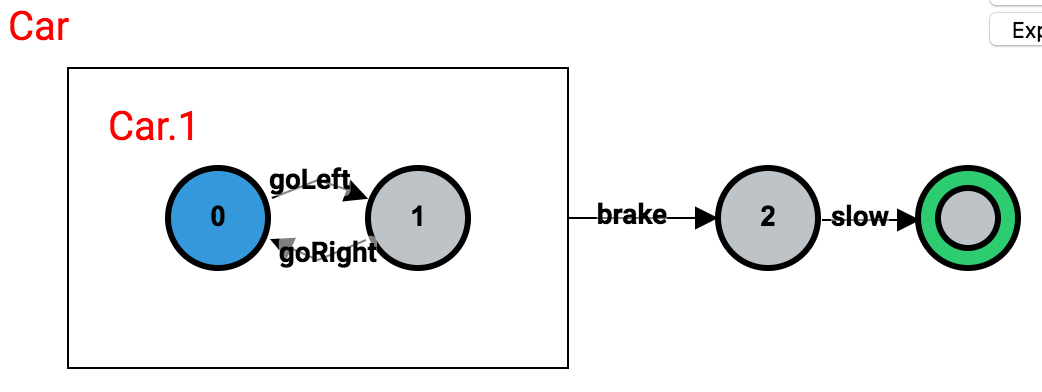
\includegraphics[scale=0.4]{InterruptCar.png}
\end{minipage}
%\hspace{\fill}


 The interrupt can be hidden. Or put another way we can remove the interrupt and express the same behaviour but at the expense of adding one {\sf brake} event per state in the original process. In this example, there are only two states in the original {\sf Steer} process.


\noindent\begin{center}\begin{minipage}{0.3\textwidth}
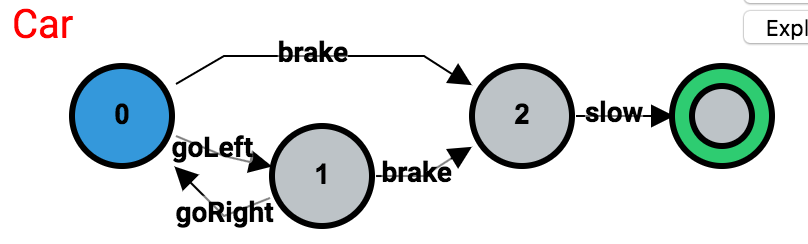
\includegraphics[scale=0.4]{InterruptCarHide.png}
\end{minipage}\end{center}

As the number of states in the initial process increases the clutter in the diagram with the interrupts hidden grows and consequently the difficulty both in specifying the hidden interrupt and understanding it grows.


\subsection{Resume} after the interrupt has finished the original process should resume from the state from which it was interrupted!

\subsection{Restart} after the interrupt has finished the original process should restart from its initial state!

}



